% latex uft-8
\documentclass[uplatex,a4paper,11pt,oneside,openany]{jsbook}
%
\usepackage[dvipdfmx]{graphicx}
\usepackage[dvipdfmx]{color}
\usepackage{svg}
\usepackage{amsmath,amssymb}
\usepackage{fancybox}
\usepackage{framed}
\usepackage{bm}
\usepackage{enumerate}
\usepackage{ascmac}
\usepackage{setspace}
\usepackage{here}
\usepackage{comment}
\usepackage{listings,jlisting} %日本語のコメントアウトをする場合jlistingが必要
%ここからソースコードの表示に関する設定
\usepackage{xcolor}

\definecolor{mygreen}{rgb}{0,0.6,0}
\definecolor{mygray}{rgb}{0.5,0.5,0.5}
\definecolor{mymauve}{rgb}{0.58,0,0.82}

\begin{comment}
\lstset{
  backgroundcolor=\color{white},   % choose the background color; you must add \usepackage{color} or \usepackage{xcolor}; should come as last argument
  basicstyle=\footnotesize,        % the size of the fonts that are used for the code
  breakatwhitespace=false,         % sets if automatic breaks should only happen at whitespace
  breaklines=true,                 % sets automatic line breaking
  captionpos=b,                    % sets the caption-position to bottom
  commentstyle=\color{mygreen},    % comment style
  deletekeywords={...},            % if you want to delete keywords from the given language
  escapeinside={\%*}{*)},          % if you want to add LaTeX within your code
  extendedchars=true,              % lets you use non-ASCII characters; for 8-bits encodings only, does not work with UTF-8
  firstnumber=1000,                % start line enumeration with line 1000
  frame=single,	                   % adds a frame around the code
  keepspaces=true,                 % keeps spaces in text, useful for keeping indentation of code (possibly needs columns=flexible)
  keywordstyle=\color{blue},       % keyword style
  language=Octave,                 % the language of the code
  morekeywords={*,...},            % if you want to add more keywords to the set
  numbers=left,                    % where to put the line-numbers; possible values are (none, left, right)
  numbersep=5pt,                   % how far the line-numbers are from the code
  numberstyle=\tiny\color{mygray}, % the style that is used for the line-numbers
  rulecolor=\color{black},         % if not set, the frame-color may be changed on line-breaks within not-black text (e.g. comments (green here))
  showspaces=false,                % show spaces everywhere adding particular underscores; it overrides 'showstringspaces'
  showstringspaces=false,          % underline spaces within strings only
  showtabs=false,                  % show tabs within strings adding particular underscores
  stepnumber=2,                    % the step between two line-numbers. If it's 1, each line will be numbered
  stringstyle=\color{mymauve},     % string literal style
  tabsize=2,	                   % sets default tabsize to 2 spaces
  title=\lstname                   % show the filename of files included with \lstinputlisting; also try caption instead of title
}
\end{comment}

%ここからソースコードの表示に関する設定

\lstdefinestyle{customc}{
  belowcaptionskip=1\baselineskip,
  breaklines=true,
  numbers=left,
  frame=single,
  xleftmargin=\parindent,
  language=C,
  showstringspaces=false,
  basicstyle=\footnotesize\ttfamily,
  keywordstyle=\bfseries\color{green!40!black},
  commentstyle=\itshape\color{purple!40!black},
  identifierstyle=\color{blue},
  stringstyle=\color{orange},
}

\lstdefinestyle{custompython}{
  belowcaptionskip=1\baselineskip,
  breaklines=true,
  numbers=left,
  frame=single,
  xleftmargin=\parindent,
  language=Python,
  showstringspaces=false,
  basicstyle=\footnotesize\ttfamily,
  keywordstyle=\bfseries\color{green!40!black},
  commentstyle=\itshape\color{purple!40!black},
  identifierstyle=\color{blue},
  stringstyle=\color{orange},
}

\lstdefinestyle{customjava}{
  belowcaptionskip=1\baselineskip,
  breaklines=true,
  numbers=left,
  frame=single,
  xleftmargin=\parindent,
  language=java,
  showstringspaces=false,
  basicstyle=\footnotesize\ttfamily,
  keywordstyle=\bfseries\color{green!40!black},
  commentstyle=\itshape\color{purple!40!black},
  identifierstyle=\color{blue},
  stringstyle=\color{orange},
}

\lstdefinestyle{customasm}{
  belowcaptionskip=1\baselineskip,
  frame=L,
  xleftmargin=\parindent,
  language=[x86masm]Assembler,
  basicstyle=\footnotesize\ttfamily,
  commentstyle=\itshape\color{purple!40!black},
}

\lstset{escapechar=@,style=custompython}

\makeatletter
\def\ps@plainfoot{%
  \let\@mkboth\@gobbletwo
  \let\@oddhead\@empty
  \def\@oddfoot{\normalfont\hfil-- \thepage\ --\hfil}%
  \let\@evenhead\@empty
  \let\@evenfoot\@oddfoot}
  \let\ps@plain\ps@plainfoot
\renewcommand{\chapter}{%
  \if@openright\cleardoublepage\else\clearpage\fi
  \global\@topnum\z@
  \secdef\@chapter\@schapter}
\makeatother
%
\newcommand{\maru}[1]{{\ooalign{%
\hfil\hbox{$\bigcirc$}\hfil\crcr%
\hfil\hbox{#1}\hfil}}}
%
\setlength{\textwidth}{\fullwidth}
\setlength{\textheight}{40\baselineskip}
\addtolength{\textheight}{\topskip}
\setlength{\voffset}{-0.55in}
%
\newenvironment{longshadowbox}{%
  \def\FrameCommand{\fboxsep=\FrameSep \shadowbox}%
  \MakeFramed {\FrameRestore}}%
 {\endMakeFramed}
%
\begin{document}
% START DOCUMENT
%
% COVER
\begin{center}
  \huge \par
  \vspace{65mm}
  \huge  \par
  \vspace{15mm}
  \LARGE 電位分布(高校生のための) \par
  \vspace{100mm}
  \Large \today \par
  \vspace{15mm}
  \Large S.Matoike \par
  \vspace{10mm}
  \Large \par
  \vspace{10mm}
\end{center}
\thispagestyle{empty}
\clearpage
\addtocounter{page}{-1}
\newpage
\setcounter{tocdepth}{3}
%
\tableofcontents
%

\chapter{電位の分布}

\section{実験の目的}

\section{実験}

\begin{itemize}
\item[実験1] 直流安定化電源の$+5$[V]とGNDの端子に接続した「棒」を電極として電場を作る
\item[実験2] 直流安定化電源の$+5$[V]とGNDの端子に接続した「板」を電極として電場を作る
\item[実験3] $+5$[V],GND,$-5$[V]の3つの電圧端子を用意し、「棒」と「板」を電極として電場を作る\\
格子点上の電位分布を測定し、等電位線を作図する。また、電場(電界)の強さと向きも求める
\end{itemize}

\subsection{実験の手順}

実験1の場合の手順は次の通り(実験2と実験3の手順は各自で)

\begin{enumerate}
  \item バットに水道の水を張って、浅い水槽をつくる
  \item 直流安定化電源の出力が+5[V]となるように、回路計の値を読みながら調整する
  \item 直流安定化電源の$+5$[V]とGNDの端子を、電極にする棒と接続し水槽に立てる
  \item 格子点の電位を回路計の値を読んで記録する
  \item 等電位線を作図する
\end{enumerate}

\subsection{-5[V]を作るには}

2台の直流安定化電源装置を使って、+5[V]、0[V]、ー5[V] の3つの電極を作る方法を考えてみます
(実験3のために必要になる)

\newpage

\subsection{等電位面(線)の作図}

例として、$v=1.75$[V]の等電位面(線)を作図する場合の手順を説明します

\begin{enumerate}
  \item $v=1.75$[V]が存在すると思われる格子線を見つけます
  \item その格子線の端点で測定した電圧の値を見て、\\
  電圧の小さい方の端点の電圧をa[V]、
  大きい方の端点の電圧をb[V]とします
  \item 格子線の長さLは、この実験では共通です。実際に測定して求めます $L=$   [mm]
  \item 比例配分によって、当該格子線上の$v=1.75$[V]の場所$x$[mm]を求めます(a$\textless$ v $\textless$ b)
  \begin{equation*}x=\frac{v-a}{b-a}\times L\end{equation*}
  \item 電圧の小さい方の点 a から $x$[mm] 離れた格子線上の点を $v=1.75$[V] の場所としてプロットします。
  この場合、 $x$ は必ず0$\textless$ x $\textless$ L になります
\end{enumerate}

格子面上に$v=1.75$[V]の所在が無くなるまで上記を繰り返し、見つけた点を直線で順に接続していくと、それが$v=1.75$[V]の等電位面(線)になります。
等電位面(線)は、$0$[V]〜$5$[V]を、$0.25$[V]間隔(大変なら$0.5$[V]間隔でもいいかな)で描くことにします。

\begin{figure}[H]
  \centering
  \begin{tabular}{ll}
      \begin{minipage}[t]{0.9\hsize}
        \centering
  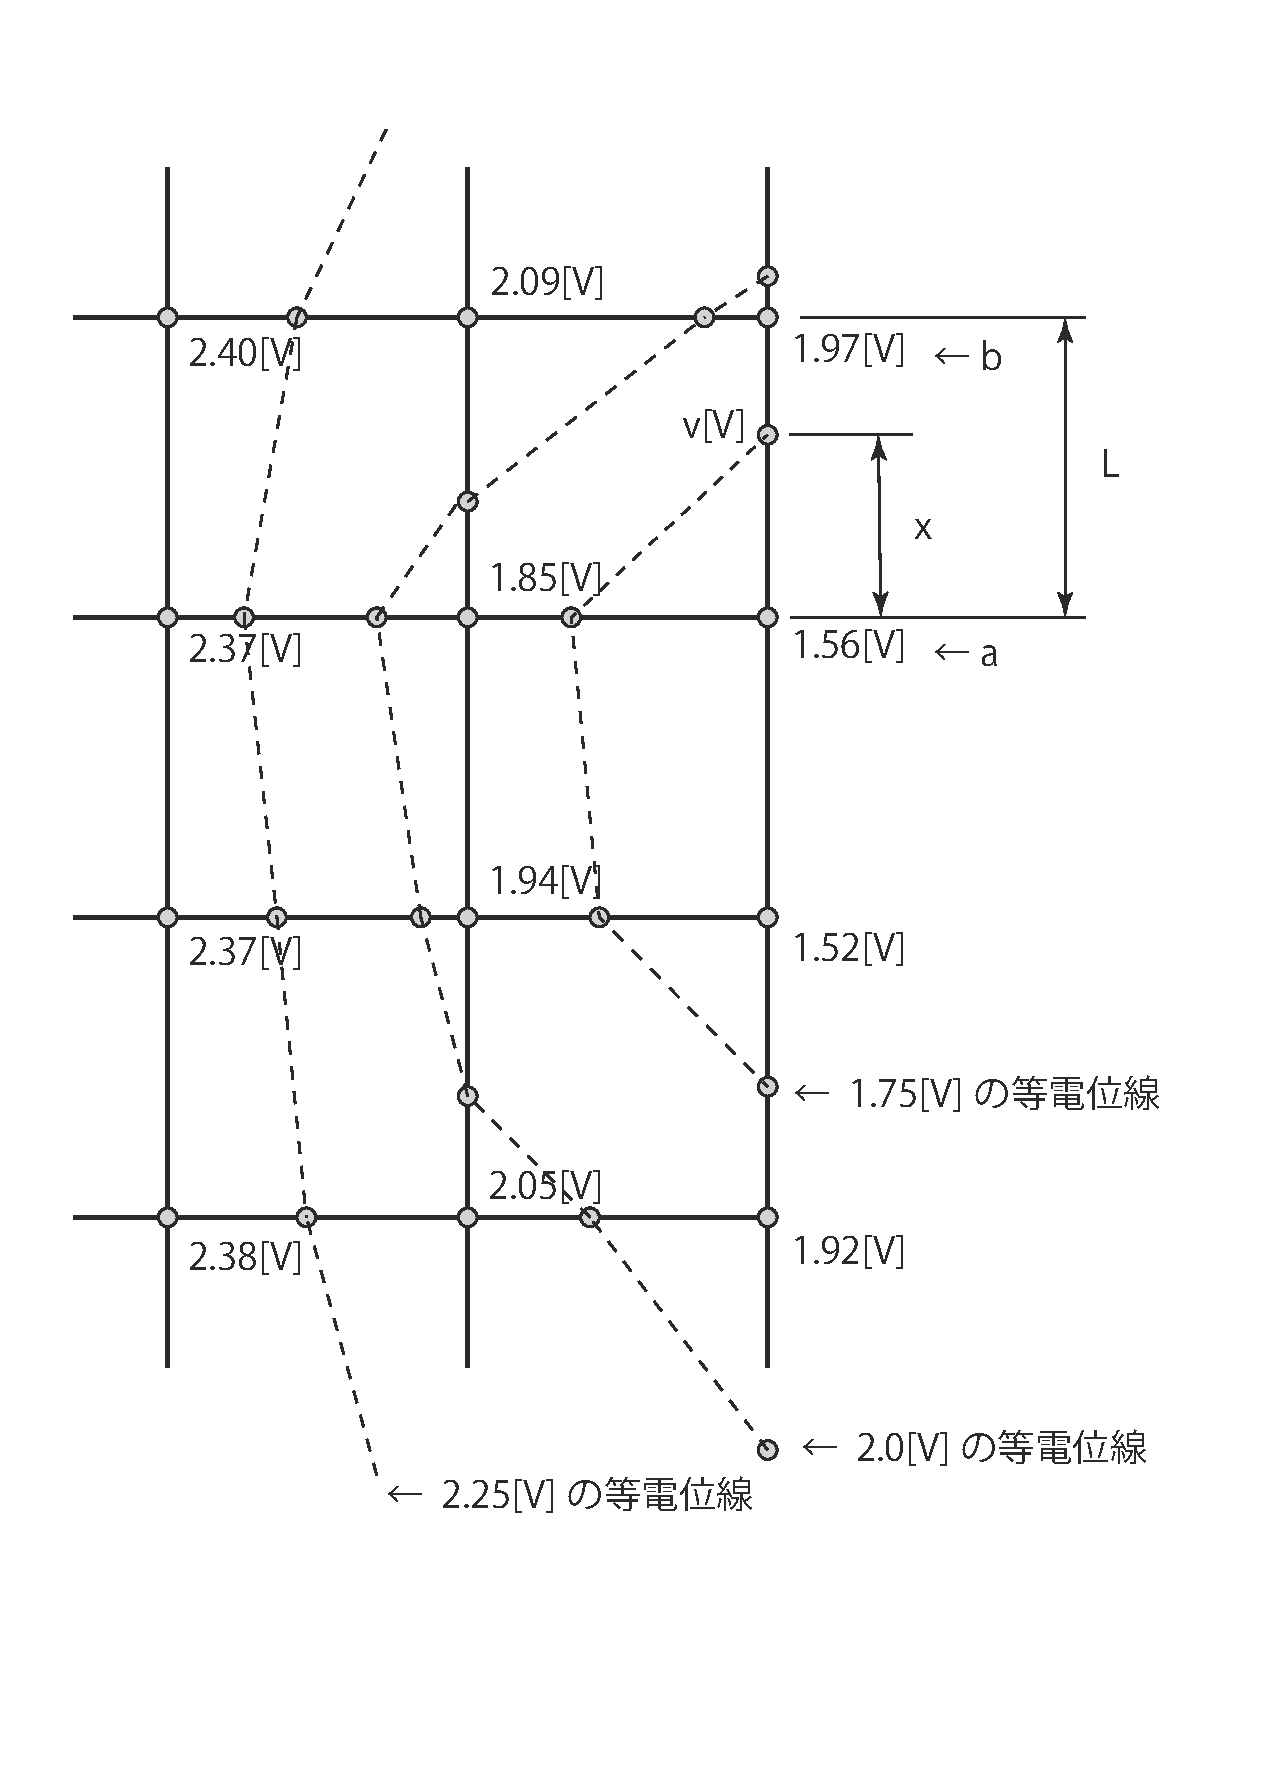
\includegraphics[scale=0.43]{./figure/potential.pdf}
      \end{minipage}
      \begin{minipage}[t]{0.1\hsize}
      %\centering
      %\begin{equation*}
      %  x = \frac{v-a}{b-a} \times L
      %\end{equation*}
%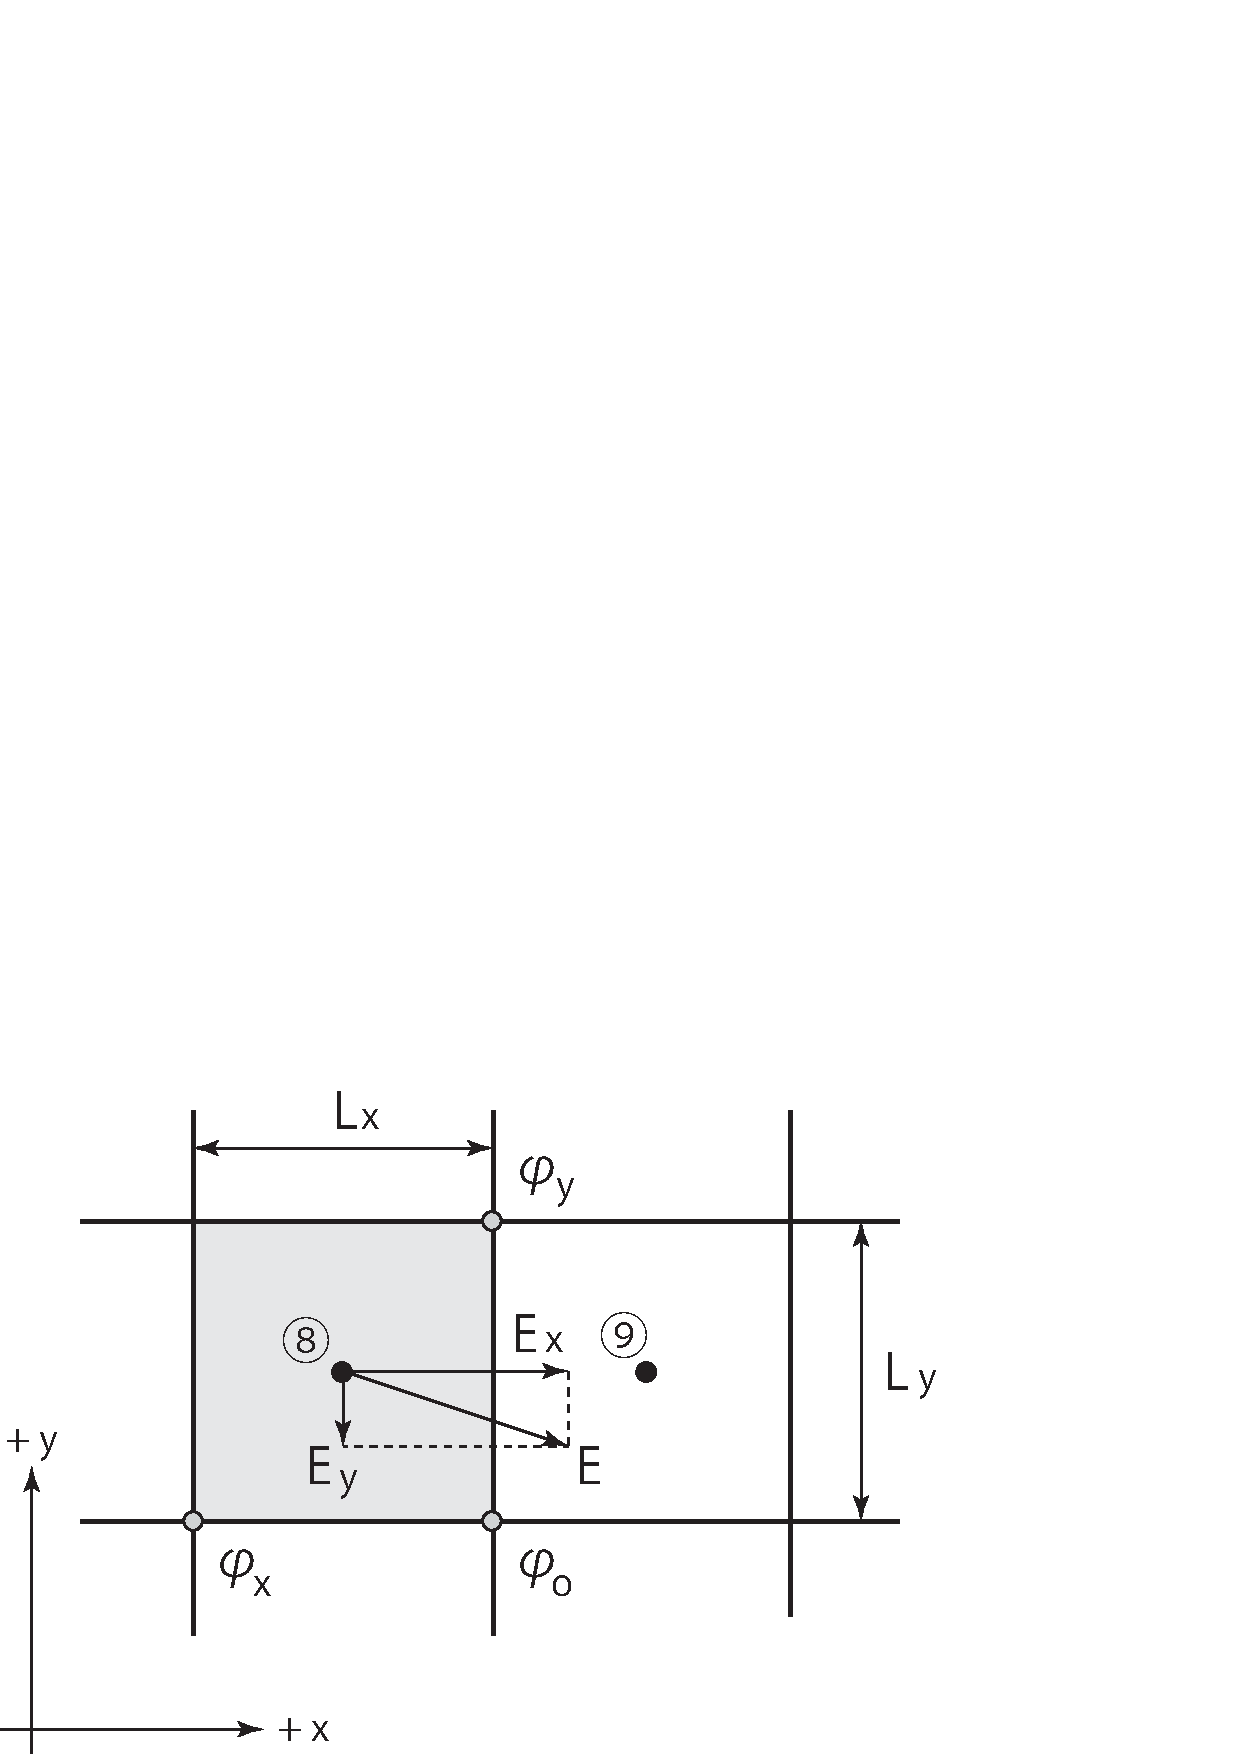
\includegraphics[scale=0.4]{field.pdf}
      \end{minipage}
    \end{tabular}
\end{figure}%

\newpage

%\centering
\begin{figure}[H]
  \centering
  \begin{tabular}{ll}
      \begin{minipage}{0.5\hsize}
        \centering
        %\begin{figure}[!h]
        %  \centering
        %  \includesvg{contr1.svg}
        %  \caption{svg image}\label{fig:example-tex}
        %\end{figure}
        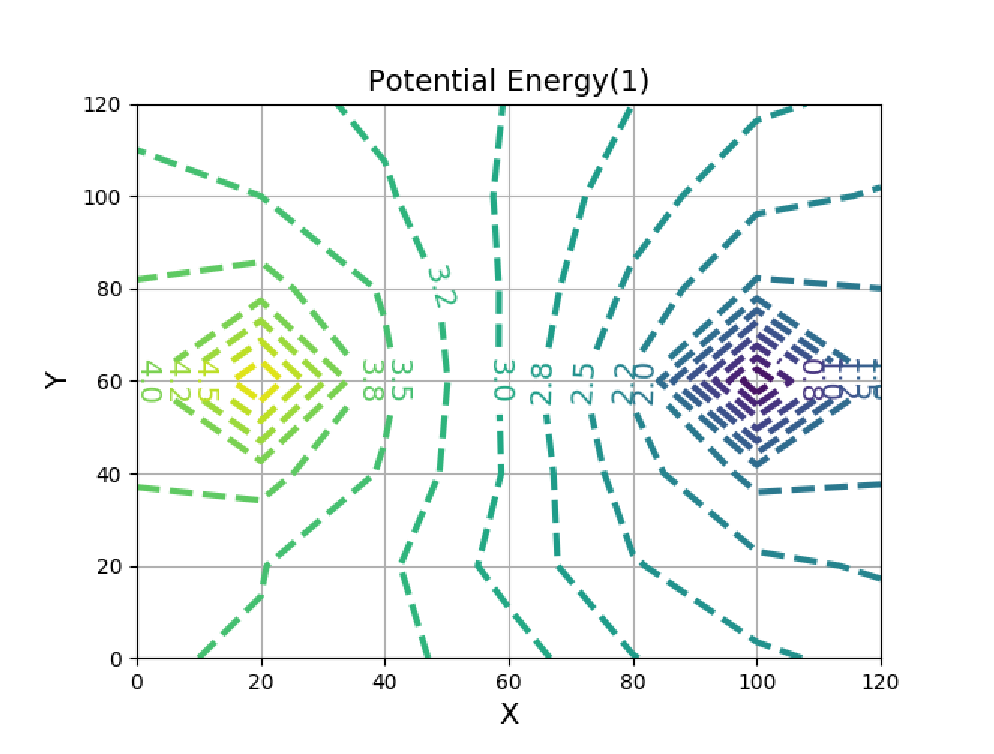
\includegraphics[scale=0.5]{./figure/contr1.eps}
      \end{minipage}
      \begin{minipage}{0.5\hsize}
        \centering
        %\begin{figure}[!h]
        %  \centering
        %  \includesvg{contr2.svg}
        %  \caption{svg image}\label{fig:example-tex}
        %\end{figure}
        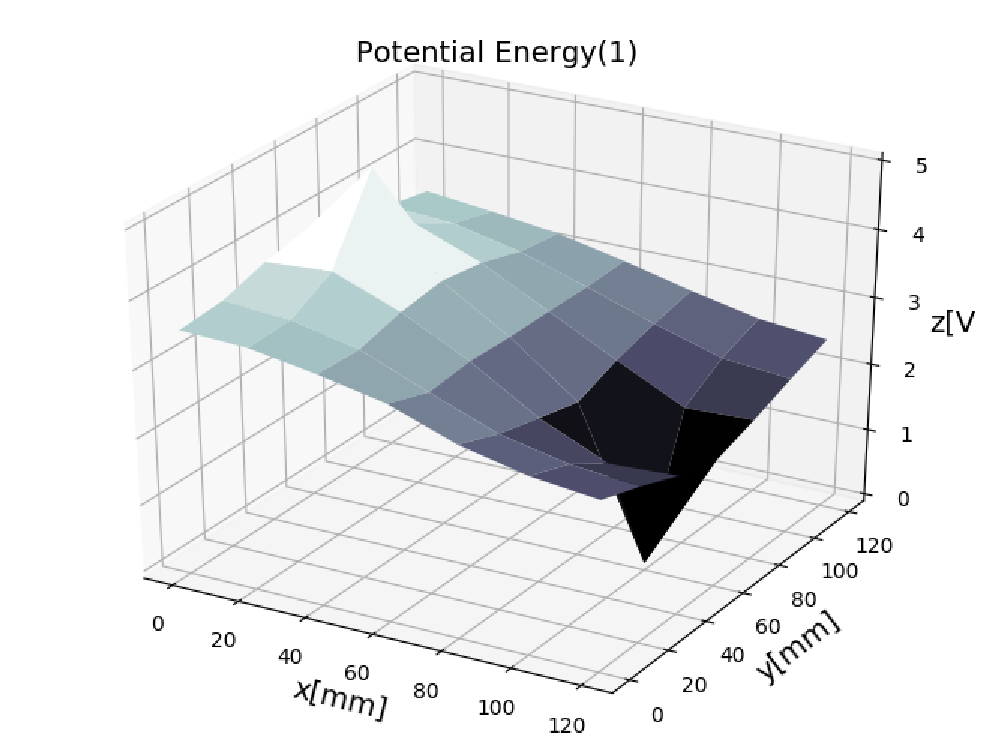
\includegraphics[scale=0.5]{./figure/contr2.eps}
      \end{minipage}
    \end{tabular}
\end{figure}
\vfill
\begin{figure}[H]
  \centering
  \begin{tabular}{ll}
      \begin{minipage}{0.5\hsize}
        \centering
        %\begin{figure}[!h]
        %  \centering
        %  \includesvg{contr1.svg}
        %  \caption{svg image}\label{fig:example-tex}
        %\end{figure}
        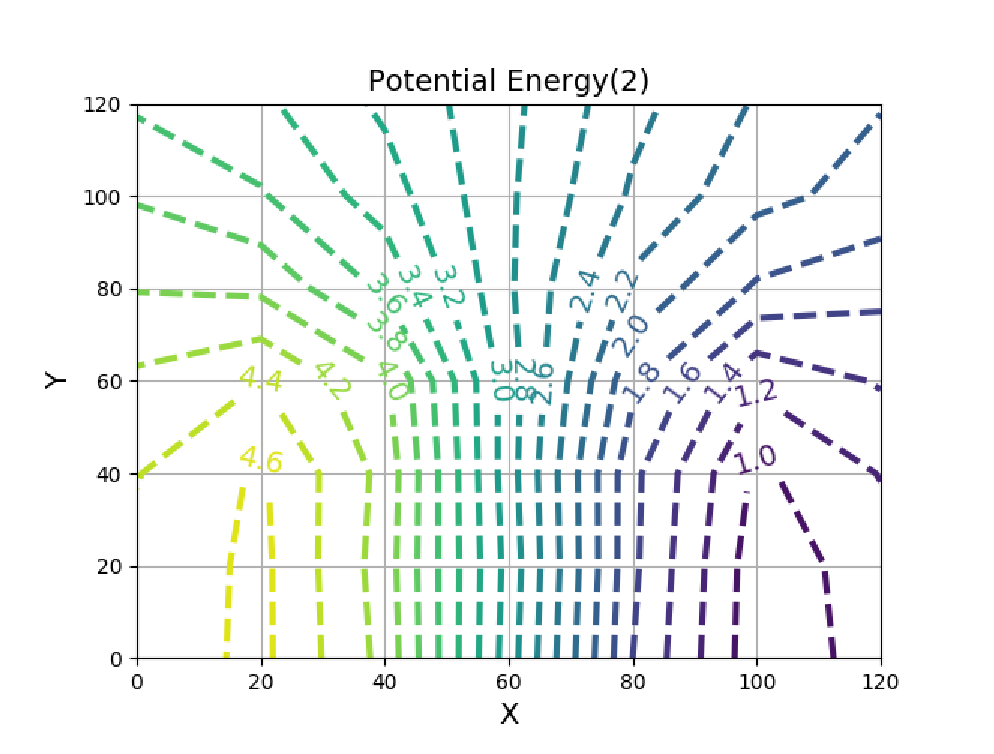
\includegraphics[scale=0.5]{./figure/contr3.eps}
      \end{minipage}
      \begin{minipage}{0.5\hsize}
        \centering
        %\begin{figure}[!h]
        %  \centering
        %  \includesvg{contr2.svg}
        %  \caption{svg image}\label{fig:example-tex}
        %\end{figure}
        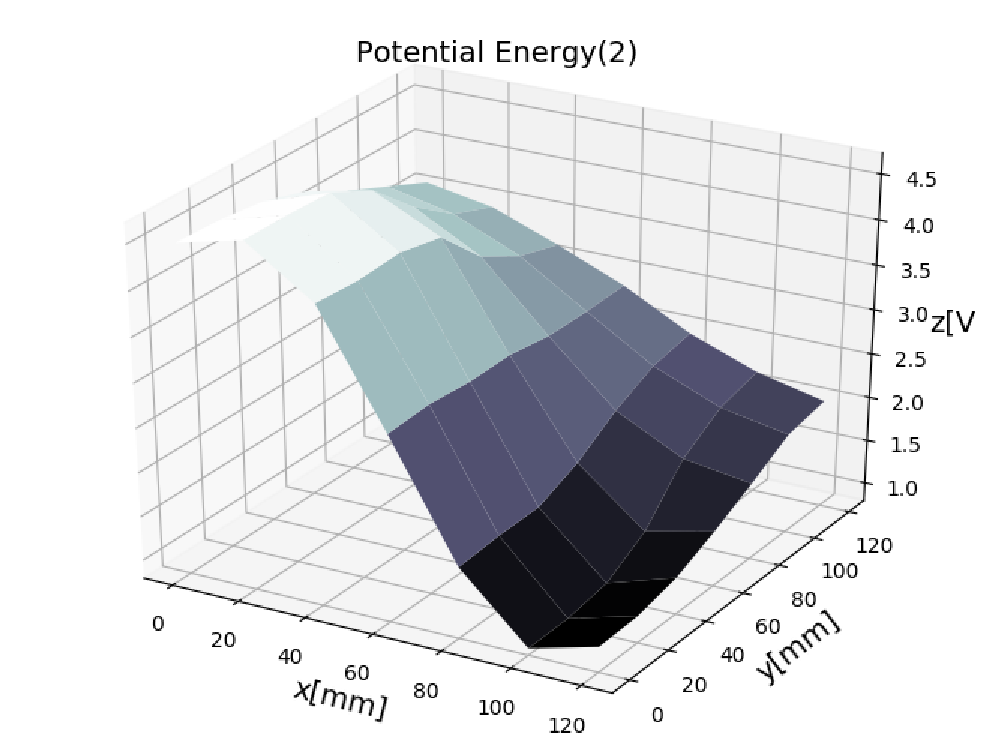
\includegraphics[scale=0.5]{./figure/contr4.eps}
      \end{minipage}
    \end{tabular}
\end{figure}
\vfill
\begin{figure}[H]
  \centering
  \begin{tabular}{ll}
      \begin{minipage}{0.5\hsize}
        \centering
        %\begin{figure}[!h]
        %  \centering
        %  \includesvg{contr1.svg}
        %  \caption{svg image}\label{fig:example-tex}
        %\end{figure}
        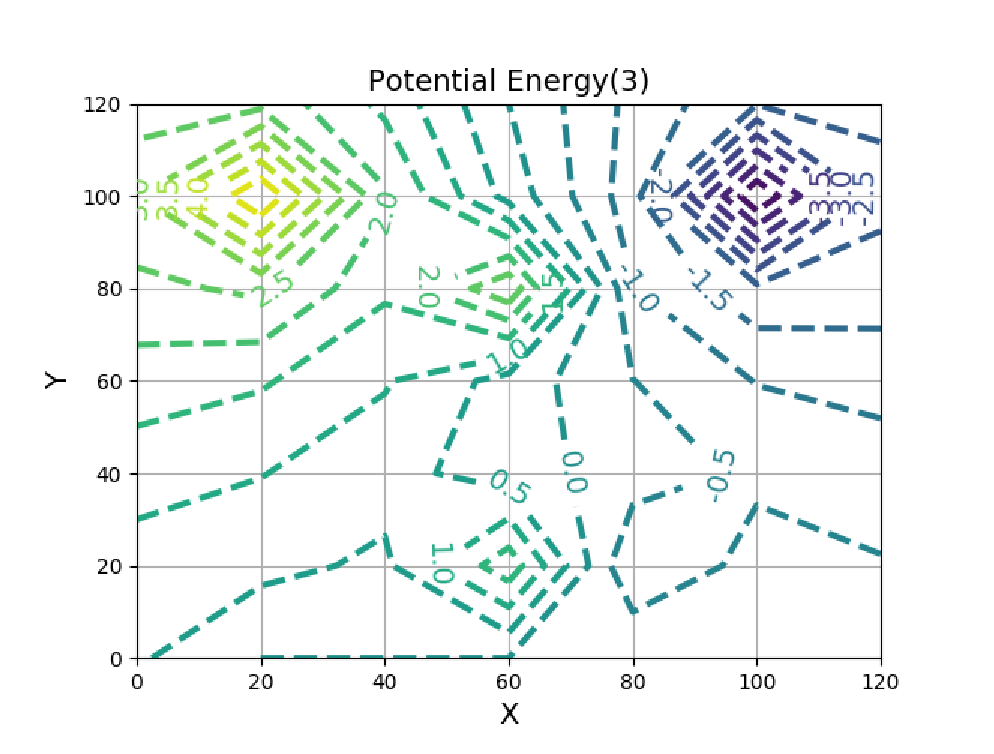
\includegraphics[scale=0.5]{./figure/contr5.eps}
      \end{minipage}
      \begin{minipage}{0.5\hsize}
        \centering
        %\begin{figure}[!h]
        %  \centering
        %  \includesvg{contr2.svg}
        %  \caption{svg image}\label{fig:example-tex}
        %\end{figure}
        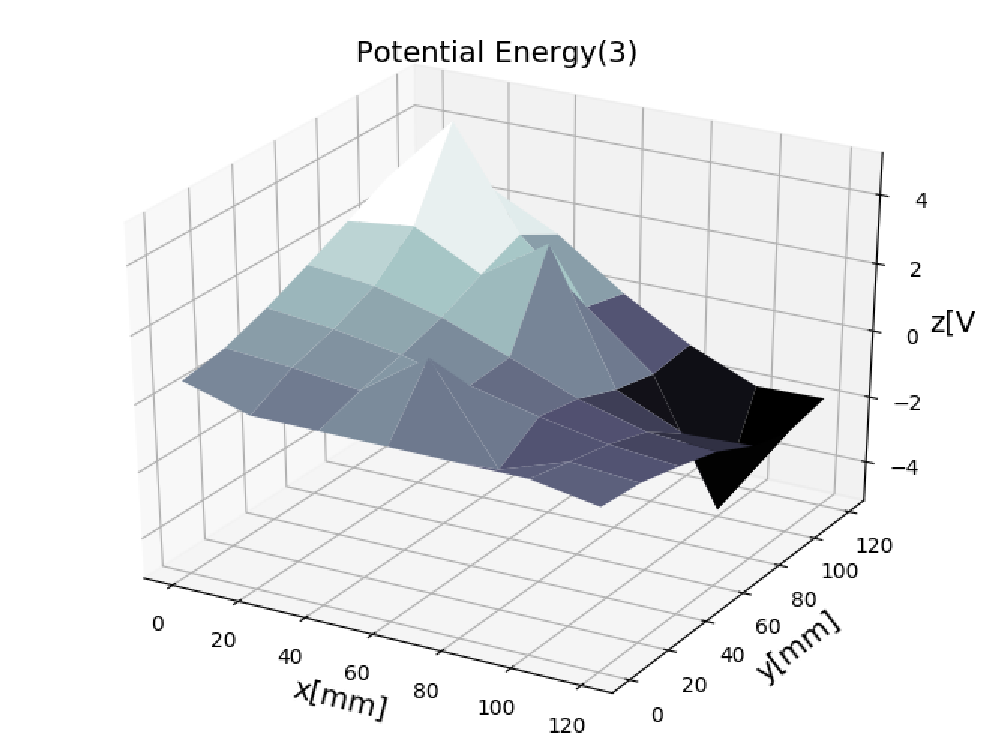
\includegraphics[scale=0.5]{./figure/contr6.eps}
      \end{minipage}
    \end{tabular}
\end{figure}%

\chapter{電界の強さと方向}

\begin{longshadowbox}
予め何らかの方法によって作られた電気の力の場(電界)がある。
その場の中に1[Coulomb]の電荷を置いた。
この時、その電荷が受ける力の大きさが$E$[Newton]であったとすると、
その電荷を置いた場所$\bm{x}(x,y)$における電界の強さは
$\bm{E}(\bm{x})$[Newton/Coulomb]であると言う。
\end{longshadowbox}

場所$\bm{x}(x,y)$における電界の強さは、その周囲の電位$\phi(\bm{x})$の様子から知ることができる。
具体的には、場所$\bm{x}(x,y)$の周辺における
電位$\phi(\bm{x})$の変化が大きいほど、その場所に置いた電荷が受ける力(=電界の強さ)が大きい。
逆に、その場所$\bm{x}(x,y)$の周辺の電位$\phi(\bm{x})$の変化が小さい場合には、
その場所に置いた電荷が受ける力(=電界の強さ)は小さい。

また、電界から電荷が力を受けると、電荷はその力の方向に向かって動かされる事になる。
この電荷の動きは、電流の流れに他ならない。
電位の変化の無い(=電位が等しい)場所では、
電荷が受ける力(=電界の強さ)はゼロであるため電流は流れない。

\section{電流の流れる方向}

実験を行った格子面上で、例として⑧の場所における電界の強さと方向を求める手順を見てみよう。

格子面上の⑧の場所$\bm{x}(x,y)$における電位$\phi(\bm{x})$の変化を、
⑧の周辺における電位の測定値である$\phi_0$、$\phi_x$、$\phi_y$ を使って近似的に求めることにする。

まず、電界の強さ$E$の$x$方向成分である$E_x(x)$について考えることにしよう。
$x$方向(横方向)の電位の変化は、近傍の2つの格子点($y$座標は同じだが$x$座標は隣り合う格子点)上の電位、
$\phi_x$と$\phi_0$の差、(即ち$\phi_0 - \phi_x$)によって知ることにする。
次に、電界の強さ$E$の$y$方向成分である$E_y(y)$について考えると、
$y$方向(縦方向)の電位の変化は、近傍の2つの格子点($x$座標は同じだが$y$座標は隣り合う格子点)上の電位、
$\phi_y$と$\phi_0$の差、(即ち$\phi_y - \phi_0$)によって知ることにする。

電位の差が同じ大きさであったとしても、それが短い距離の間で急に生じている変化量なのか、
長い格子間隔でようやく生じた変化量なのかを考えると、前者は大きな(=急激な)変化であり、
後者は小さな(=ゆるやかな)変化であると捉えることができる。

以上の考察により、
%$x$方向(横方向)の電位$\phi$の変化、及び$y$方向(縦方向)の電位$\phi$の変化によって導かれる、
電界の強さ$\bm{E}$の$x$成分$E_x$と、$y$成分$E_y$は、次の様にして求めることができる。
\begin{figure}[H]
  \centering
  \begin{tabular}{lr}
      \begin{minipage}[t]{0.4\hsize}
        %\centering
        \begin{eqnarray*}
          E_x &=& -\frac{\phi_0-\phi_x}{L_x} \\ \\
          E_y &=& -\frac{\phi_y-\phi_0}{L_y} \\ \\
          \left| E \right| &=& \sqrt{{E_x}^2 + {E_y}^2}
        \end{eqnarray*}
      \end{minipage}
      \begin{minipage}[t]{0.5\hsize}
        %\centering
        \begin{figure}[H]
  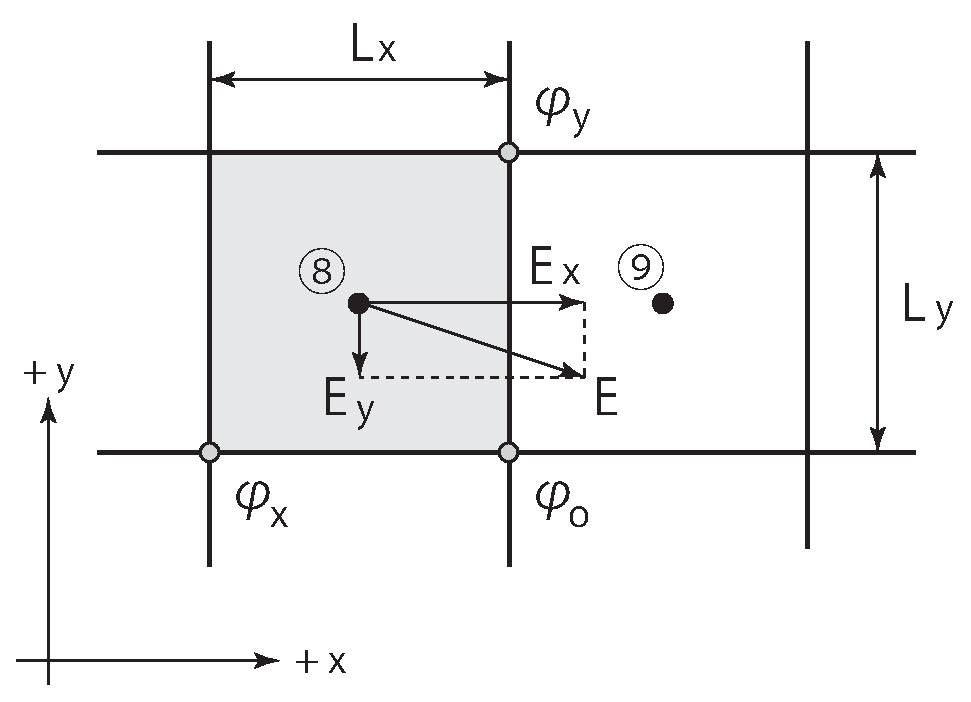
\includegraphics[clip,scale=0.45]{./figure/field.eps}
        \end{figure}
      \end{minipage}
    \end{tabular}
\end{figure}%
点⑧に置かれた1[Coulomb]の電荷は、\\
$x$方向(横方向)に$E_x$の力を受けると同時に、
$y$方向(縦方向)にも$E_y$の力を受ける。\\
その結果、電荷は$E$の方向へ動こうとする。
電荷の移動、これは即ち「電流」の流れである。\\

電界の強さは、1[Coulomb]当たりの電荷に働く力[Newton]なので、$E$の単位は[Newton/Coulomb]である。
一方これまでの考察から電界$E_x$の大きさは、$x$方向の単位長さ1メートル[Meter]当たりの電圧$\phi$[Volt]の変化量、
そして電界$E_y$の大きさも、$y$方向の単位長さ1メートル[Meter]当たりの電圧$\phi$[Volt]の変化量ですから、
$E$の単位は[Volt/Meter]と表すこともできる。

もっと正確に説明すると、
1[Volt]=1[Joule/Coulomb]を用いることによって、電界$E$の単位は、\\
1[Newton/Coulomb]=1[(Joule/Meter)/Coulomb]=1[Volt/Meter]となります。こちらの単位の方がよく使われます。\\

これまで、1[Coulomb]の電荷に対して作用する力$E$[Newton]が分布する場(電界)について考察してきたが、
$q$[Coulomb]の電荷を置いた場合は、クーロンの法則にもある通り、その電荷は$qE$[Newton]の力を受けることになる。

\newpage

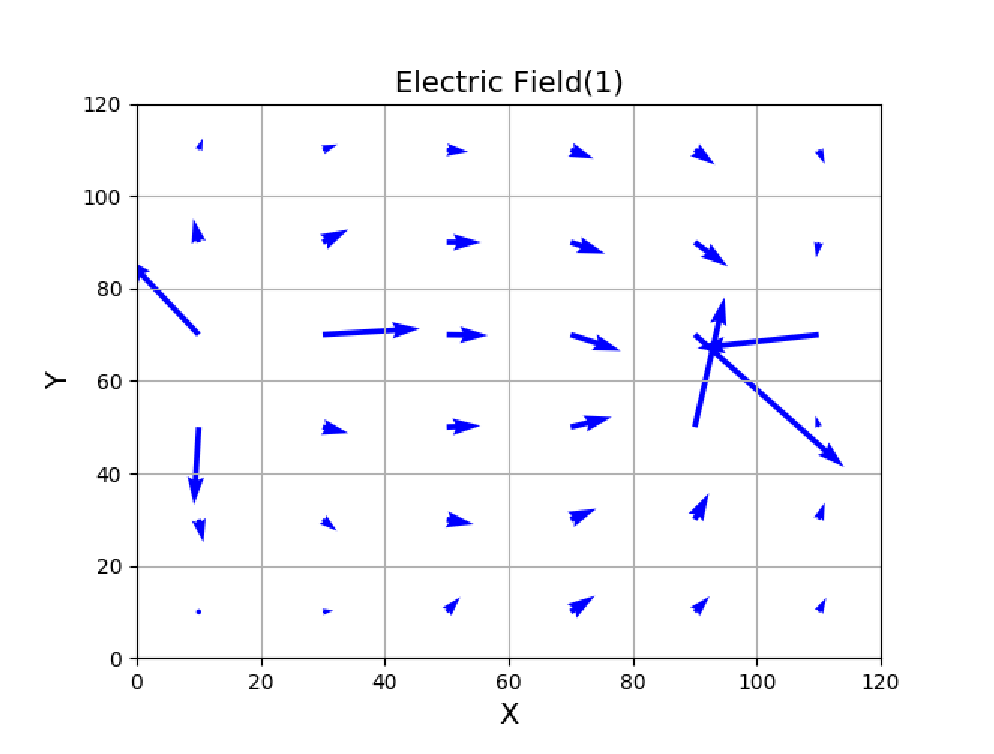
\includegraphics[scale=0.62]{./figure/Efield1.eps}
\vfill
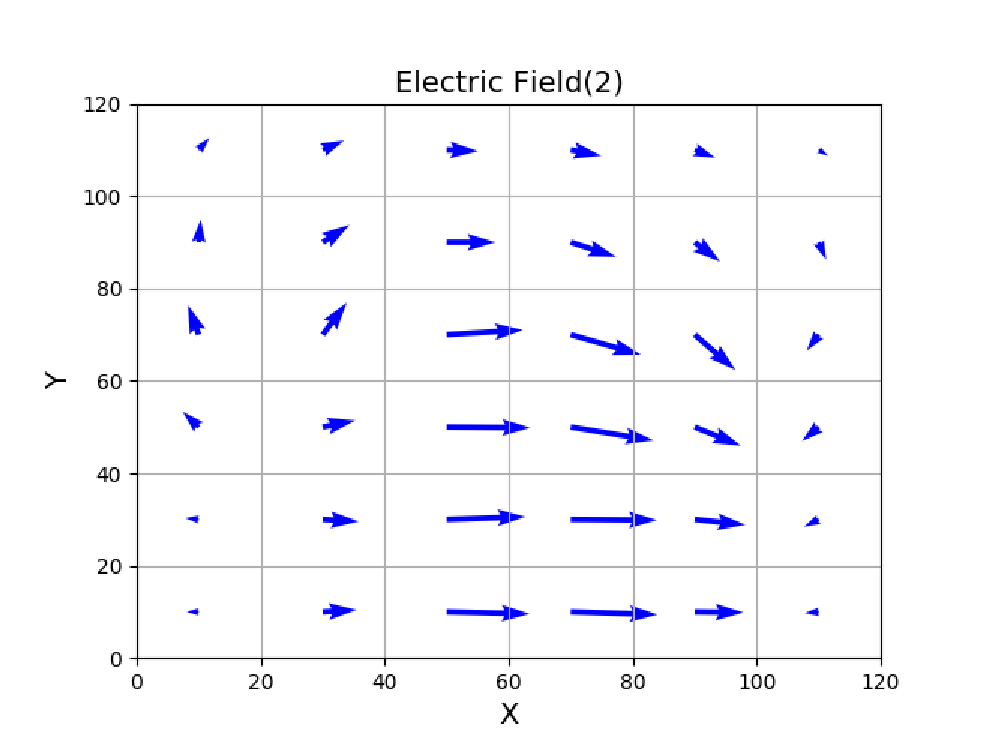
\includegraphics[scale=0.62]{./figure/Efield2.eps}
\vfill
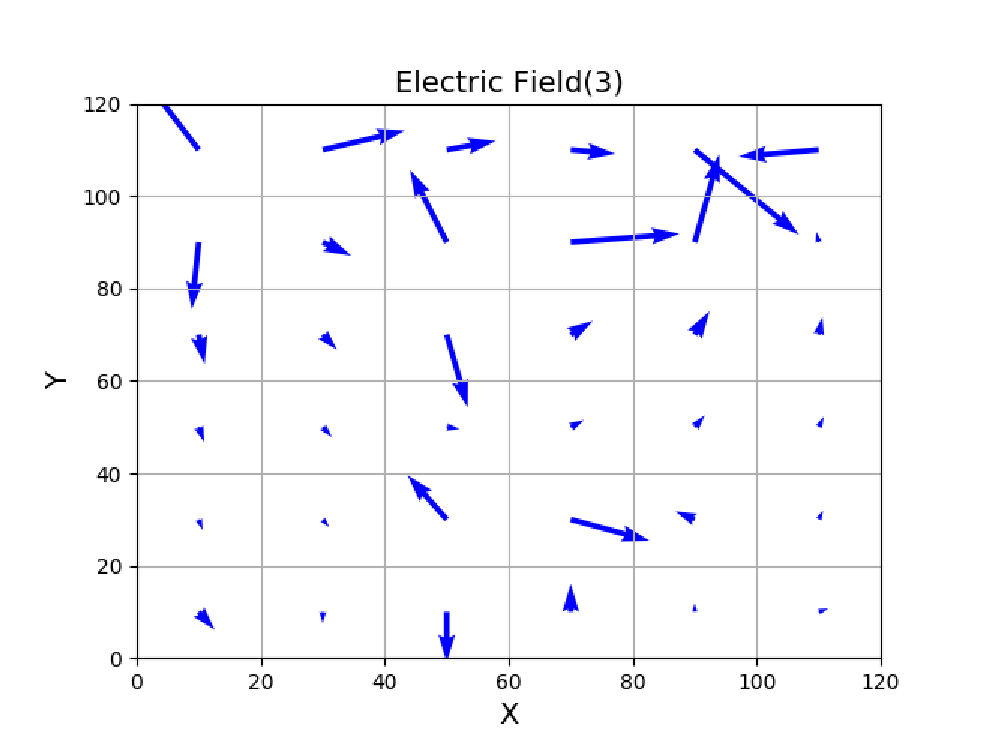
\includegraphics[scale=0.62]{./figure/Efield3.eps}

\chapter{模擬実験}

\section{格子間隔を無限に小さく(微分)}

$x$方向(横方向)の電位$\phi$の変化、及び$y$方向(縦方向)の電位$\phi$の変化は、
数学ではそれを(偏)微分の演算子を使って記述できます。
格子間隔の$L_x$や$L_y$を極限まで短くして、非常に細かな格子にしたときに
以下のような微分演算子による電場の記述が可能になります。
また、$\phi$は場所$(x,y)$によって決まる値を取る。
(このことを「$\phi$は$x$と$y$の関数である」と言い、$\phi(x,y)$と記述します)

$x$と$y$の関数である$\phi(x,y)$において、$y$を同じ値のまま変えずに$x$だけの変化量を得るには、
偏微分の演算子$\partial / \partial x$を用いて$\partial \phi/\partial x$と書きます。
同様に、$x$を同じ値のまま変えずに$y$だけの変化量を知る場合も、偏微分の演算子$\partial/\partial y$を使って$\partial \phi/\partial y$と書きます。(本実習では、$L_x$も$L_y$も長くてとても粗い格子ですが、次の式の右辺の様な大雑把な概算をして電場のイメージを描画してみたものです。)
\begin{eqnarray*}
  E_x &=& -\frac{\partial}{\partial x}\phi \thickapprox -\frac{\phi_0-\phi_x}{L_x}\\ \\
  E_y &=& -\frac{\partial}{\partial y}\phi \thickapprox -\frac{\phi_y-\phi_0}{L_y}
\end{eqnarray*}%

ここに現れた偏微分の演算子を、まとめて$\nabla$(ナブラと読む)という記号で書くことがあります。
\begin{equation*}
  \nabla = ( \frac{\partial}{\partial x}, \frac{\partial}{\partial y})
\end{equation*}%

この演算子$\nabla$を、電位$\phi$のようなスカラ量に対して作用させる場合、特に$\mathrm{grad}$(グラディエントと読む。日本語では「勾配」)という記号を使います。これを使うと、上記の電界の強さ$E_x$や$E_y$が電位$\phi$の変化量だとする式は次の様に書けます。
\begin{equation*}
  \bm{E}=\nabla (- \phi) = - \mathrm{grad} \phi
\end{equation*}%

また同じ演算子$\nabla$を、電界$\bm{E}=(E_x, E_y)$のようなベクトル量に対して作用させる場合は、
特に$\mathrm{div}$(ダイバージェンスと読む。日本語では「発散」)という記号が使われます。
例えば次の式は、電荷を内部に含む微少体積を貫いて出入りする電気力線(電界$\bm{E}$の方向と一致)の収支が、その微少体積内部の電荷量に比例するとするガウスの法則の微分形式です。($\rho$は電荷密度分布、$\varepsilon_0$は真空の誘電率、$\bm{D}$は電束密度(電気変位とも言う))
もし右辺がゼロならば、微少体積に入ってくる電気力線は、全てそのまま出て行く事になり、変化量は無し、収支ゼロになりますが、電界では収支ゼロになりません。(これを「湧きだしがある」といいます)因みに磁界の場合、磁束密度$\bm{B}$の収支はゼロになります。(つまり、$\mathrm{div}\bm{B}=0$、湧きだしなしです)
\begin{equation*}
  \nabla \bm{E} = \mathrm{div}\bm{E} = \frac{\rho}{\varepsilon_0}, \hspace*{2zw}\mathrm{div}\bm{D} = \rho \hspace*{2zw}ここで\bm{D}=\varepsilon_0 \bm{E}
\end{equation*}

$\nabla$も$\mathrm{grad}$も$\mathrm{div}$も、どれも「〜の(位置座標に関する)変化量」という意味では同じです。
つまり、$\mathrm{grad}\phi$は「$\phi$の変化量」という意味であり、$\mathrm{div}\bm{E}$は「$\bm{E}$の変化量」という意味になります。

$\mathrm{grad}$も$\mathrm{div}$も$\nabla$と同じ格好をした演算子ですから、$\mathrm{grad}$に$\mathrm{div}$を作用させることを、あたかもナブラ$\nabla$同士の内積と同じ様に扱って、形式的に演算を進めることができます。
\begin{equation*}
  \mathrm{div}\bm{E} = \mathrm{div}(-\mathrm{grad}\phi) = -\nabla \cdot \nabla \phi = -\nabla^2 \phi = -(\frac{\partial^2}{\partial x^2} + \frac{\partial^2}{\partial y^2})\phi = -\Delta \phi = \frac{\rho}{\varepsilon_0}
\end{equation*}%

演算子$\Delta$は、ラプラシアン(ラプラスの演算子)と呼ばれています。
\begin{equation*}
  \Delta = \nabla \cdot \nabla = (\frac{\partial^2}{\partial x^2}+\frac{\partial^2}{\partial y^2})
\end{equation*}%

次の式で、前者はラプラス(Laplace)の方程式、後者はポアソン(Poisson)の方程式と呼ばれています。
\begin{eqnarray*}
  \Delta \phi &=& 0\\ \\
  \Delta \phi &=& -\frac{\rho}{\varepsilon_0}
\end{eqnarray*}%


これが、電界(電場)を記述している式の1つになります。

\section{内部の点の離散化}

ここまでは実験を通して実際に測定した格子点上の電位を元に、等電位面(線)を求めてきました。

ここからは、ポアソンの方程式、あるいは電荷密度の分布していない電場を表すラプラスの方程式からスタートして、
計算機による模擬実験(シミュレーション)を行い、電位の分布つまり等電位面(線)の描画をしてみます。

計算機による模擬実験が、どの程度まで実際の現象を再現できるものなのか、
実験データによって測定した電位分布と、ラプラスの方程式を計算機で解いて求めた電位分布とを比べてみることにしましょう。

ポアソンの方程式を再掲すると次の通りです。
\begin{eqnarray*}
  -\varepsilon \Delta \phi = -\varepsilon (\frac{\partial^2}{\partial x^2}+\frac{\partial^2}{\partial y^2})\phi = \rho
\end{eqnarray*}

この方程式を計算機で解くためには、この式を離散化するという作業が必要になります。ここでは差分法による離散化を行います。

下の図に示す様に、格子点Pに着目したコントロール・ボリューム(斜線部)における収支を考えます。z方向に単位長さ1を持つ面wと、同様の面sから流入する量はそれぞれ次の様になります。
\begin{equation*}
  -\varepsilon \frac{\partial \phi}{\partial x} \mid _{w}(\varDelta y \cdot 1),\hspace*{2zw}
  -\varepsilon \frac{\partial \phi}{\partial y} \mid _{s}(\varDelta x \cdot 1)
\end{equation*}

同じ様にして、面eと面nから流出する量は、それぞれ次の通り表せます。
\begin{equation*}
  -\varepsilon \frac{\partial \phi}{\partial x} \mid _{e}(\varDelta y \cdot 1),\hspace*{2zw}
  -\varepsilon \frac{\partial \phi}{\partial y} \mid _{n}(\varDelta x \cdot 1)
\end{equation*}

この4つの総和がここで着目しているコントロール・ボリュームにおける収支であり、今はこの中に電荷分布の存在を考えていませんから、4つの総和はゼロになります。
これはラプラスの方程式ですね。
\begin{equation*}
  -\varepsilon \left\{ (\varDelta y \cdot 1)(\frac{\partial \phi}{\partial x}\mid_{w} - \frac{\partial \phi}{\partial x}\mid_{e}) + (\varDelta x \cdot 1)(\frac{\partial \phi}{\partial y}\mid_{s} - \frac{\partial \phi}{\partial y}\mid_{n}) \right\}=0
\end{equation*}

これまでの実習の中で行ってきたのと同じ様にして、この式に現れた偏微分(変化量)を、近傍の格子点の値の差を使って表すことにします。
\begin{figure}[H]
  \centering
  \begin{tabular}{lr}
      \begin{minipage}[t]{0.4\hsize}
        %\centering
        \begin{eqnarray*}
          \frac{\partial \phi}{\partial x}\mid_{w}&=&\frac{\phi_{P}-\phi_{W}}{(\delta x)_{w}} \\ \\
          \frac{\partial \phi}{\partial x}\mid_{e}&=&\frac{\phi_{E}-\phi_{P}}{(\delta x)_{e}} \\ \\
          \frac{\partial \phi}{\partial y}\mid_{s}&=&\frac{\phi_{P}-\phi_{S}}{(\delta y)_{s}} \\ \\
          \frac{\partial \phi}{\partial y}\mid_{n}&=&\frac{\phi_{N}-\phi_{P}}{(\delta y)_{n}}
        \end{eqnarray*} 
      \end{minipage}
      \begin{minipage}[t]{0.5\hsize}
        %\centering
        \begin{figure}[H]
  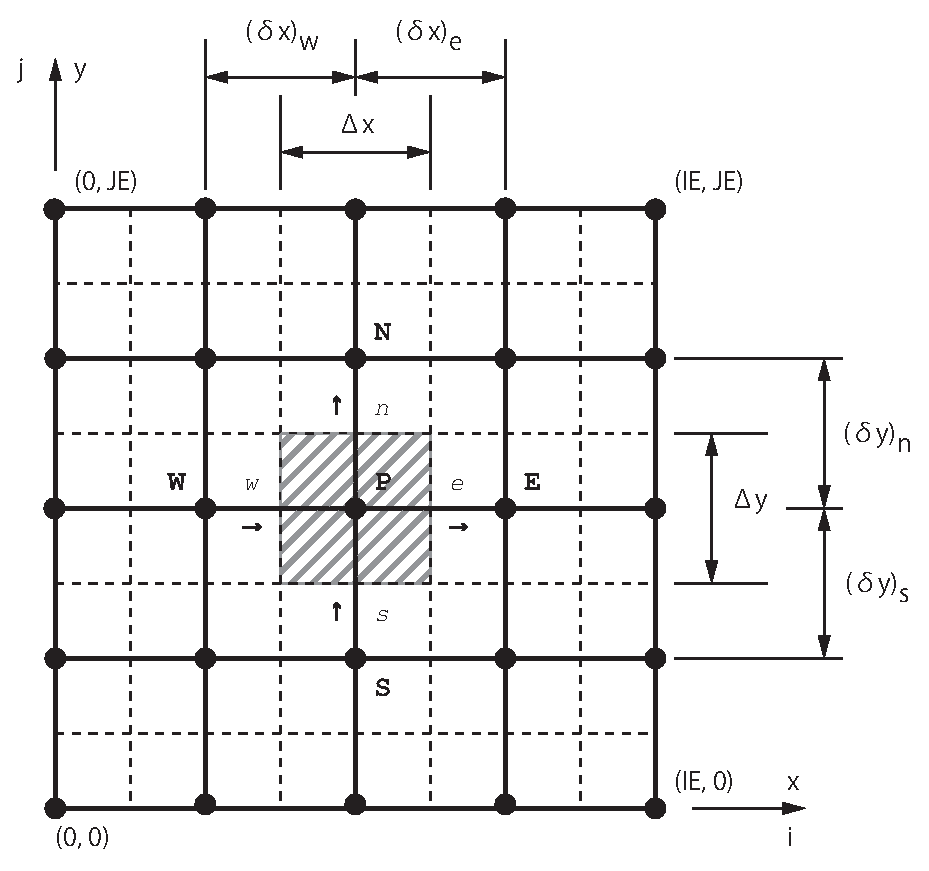
\includegraphics[clip,scale=0.45]{./figure/cvolume.eps}
        \end{figure}
      \end{minipage}
    \end{tabular}
\end{figure}%

これを先ほどの、コントロール・ボリュームにおける収支はゼロという式に代入します。ただし、
格子は規則的に設けることにして、$(\delta x)_{w}=(\delta x)_{e}=\varDelta x$、$(\delta y)_{s}=(\delta y)_{n}=\varDelta y$と
置き換えて計算を進めることにします。
\begin{equation*}
  \varDelta y(\frac{\phi_{P}-\phi_{W}}{\varDelta x}-\frac{\phi_{E}-\phi_{P}}{\varDelta x})+\varDelta x(\frac{\phi_{P}-\phi_{S}}{\varDelta y}-\frac{\phi_{N}-\phi_{P}}{\varDelta y})=0
\end{equation*}

P点の電位$\phi_{P}$について整理すると、
\begin{equation*}
  \phi_{P}=\frac{{\varDelta y}^2}{2({\varDelta x}^2+{\varDelta y}^2)}(\phi_{E}+\phi_{W})+
  \frac{{\varDelta x}^2}{2({\varDelta x}^2+{\varDelta y}^2)}(\phi_{S}+\phi_{N})
\end{equation*}

この式を見ると、P点の電位$\phi_{P}$は、P点を取り囲む東西南北の各格子点、E点の電位$\phi_{E}$、W点の電位$\phi_{W}$、S点の電位$\phi_{S}$、N点の電位$\phi_{N}$の4つから(平して)求めるという形になっています。

ここまでの状態でプログラムして計算させることもできますが、実際にはこれを次の様に、
無次元化と呼ばれる式の変形を施した上でプログラムするようにします。
\begin{equation*}
  T_{i,j} = \frac{A^2 {\varDelta Y}^2}{2({\varDelta X}^2+A^2 {\varDelta Y}^2)} (T_{i-1,j}+T_{i+1,j})+
          \frac{A^2 {\varDelta X}^2}{2({\varDelta X}^2+A^2 {\varDelta Y}^2)}(T_{i,j-1}+T_{i,j+1})
\end{equation*}

ここで、$A=y_{max}/x_{max}$(縦横比)、$\varDelta X=1/IE$、$\varDelta Y=1/JE$とします。

また、$T_{i,j}=(\phi_{i,j}-\phi_{min})/(\phi_{max}-\phi_{min})$、$X=x/x_{max}$、$Y=y/y_{max}$なので、
これによって模擬実験対象のモデルの領域は$0<X\le1$、$0<Y\le1$、$0<T\le1$の範囲で計算されることになります。

計算は、まず対象領域内部の$T_{i,j}$の初期値を適当に仮定し、次に上の式で$T_{i,j}$($i=1〜IE-1$、$j=1〜JE-1$)を順次修正していきます。
各点の値が必要な桁数に収束するまで、繰り返しこの式で格子点の値を平していくことになります。

計算結果$T_{i,j}$から元の物理量$\phi_{i,j}$を得るには、$\phi_{i,j}=T_{i,j}\times(\phi_{max}-\phi_{min})+\phi_{min}$とすれば求まります。


%\section{境界条件と式の解法}

\newpage

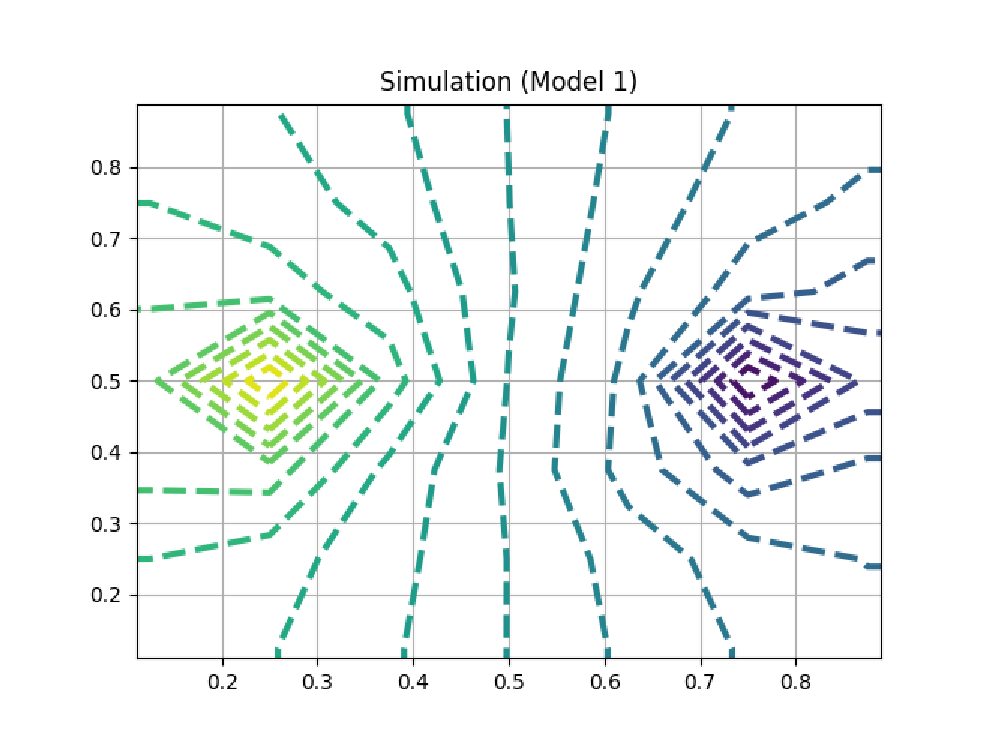
\includegraphics[scale=0.62]{./figure/simu1.eps}
\vfill
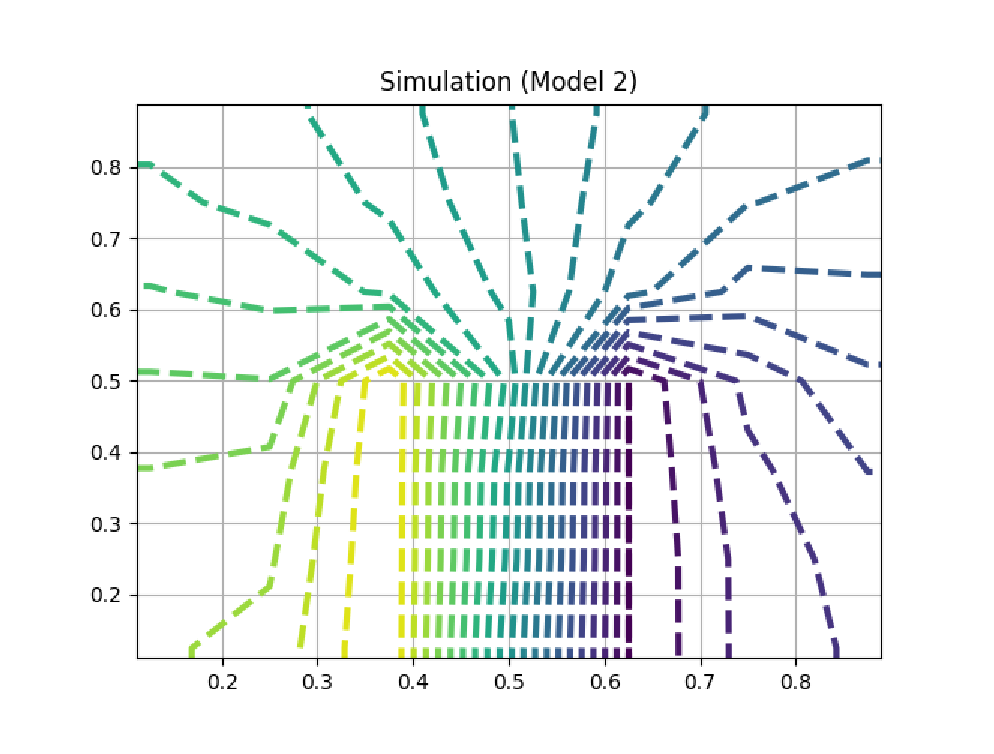
\includegraphics[scale=0.62]{./figure/simu2.eps}
\vfill
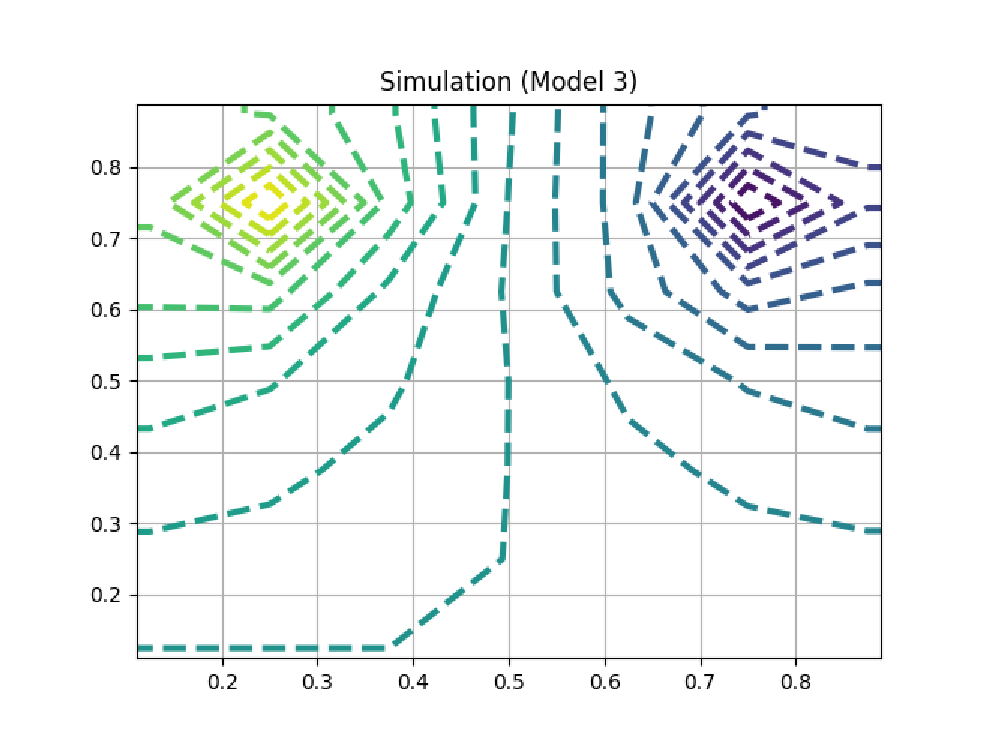
\includegraphics[scale=0.62]{./figure/simu3.eps}

\chapter{補助資料}

\newpage

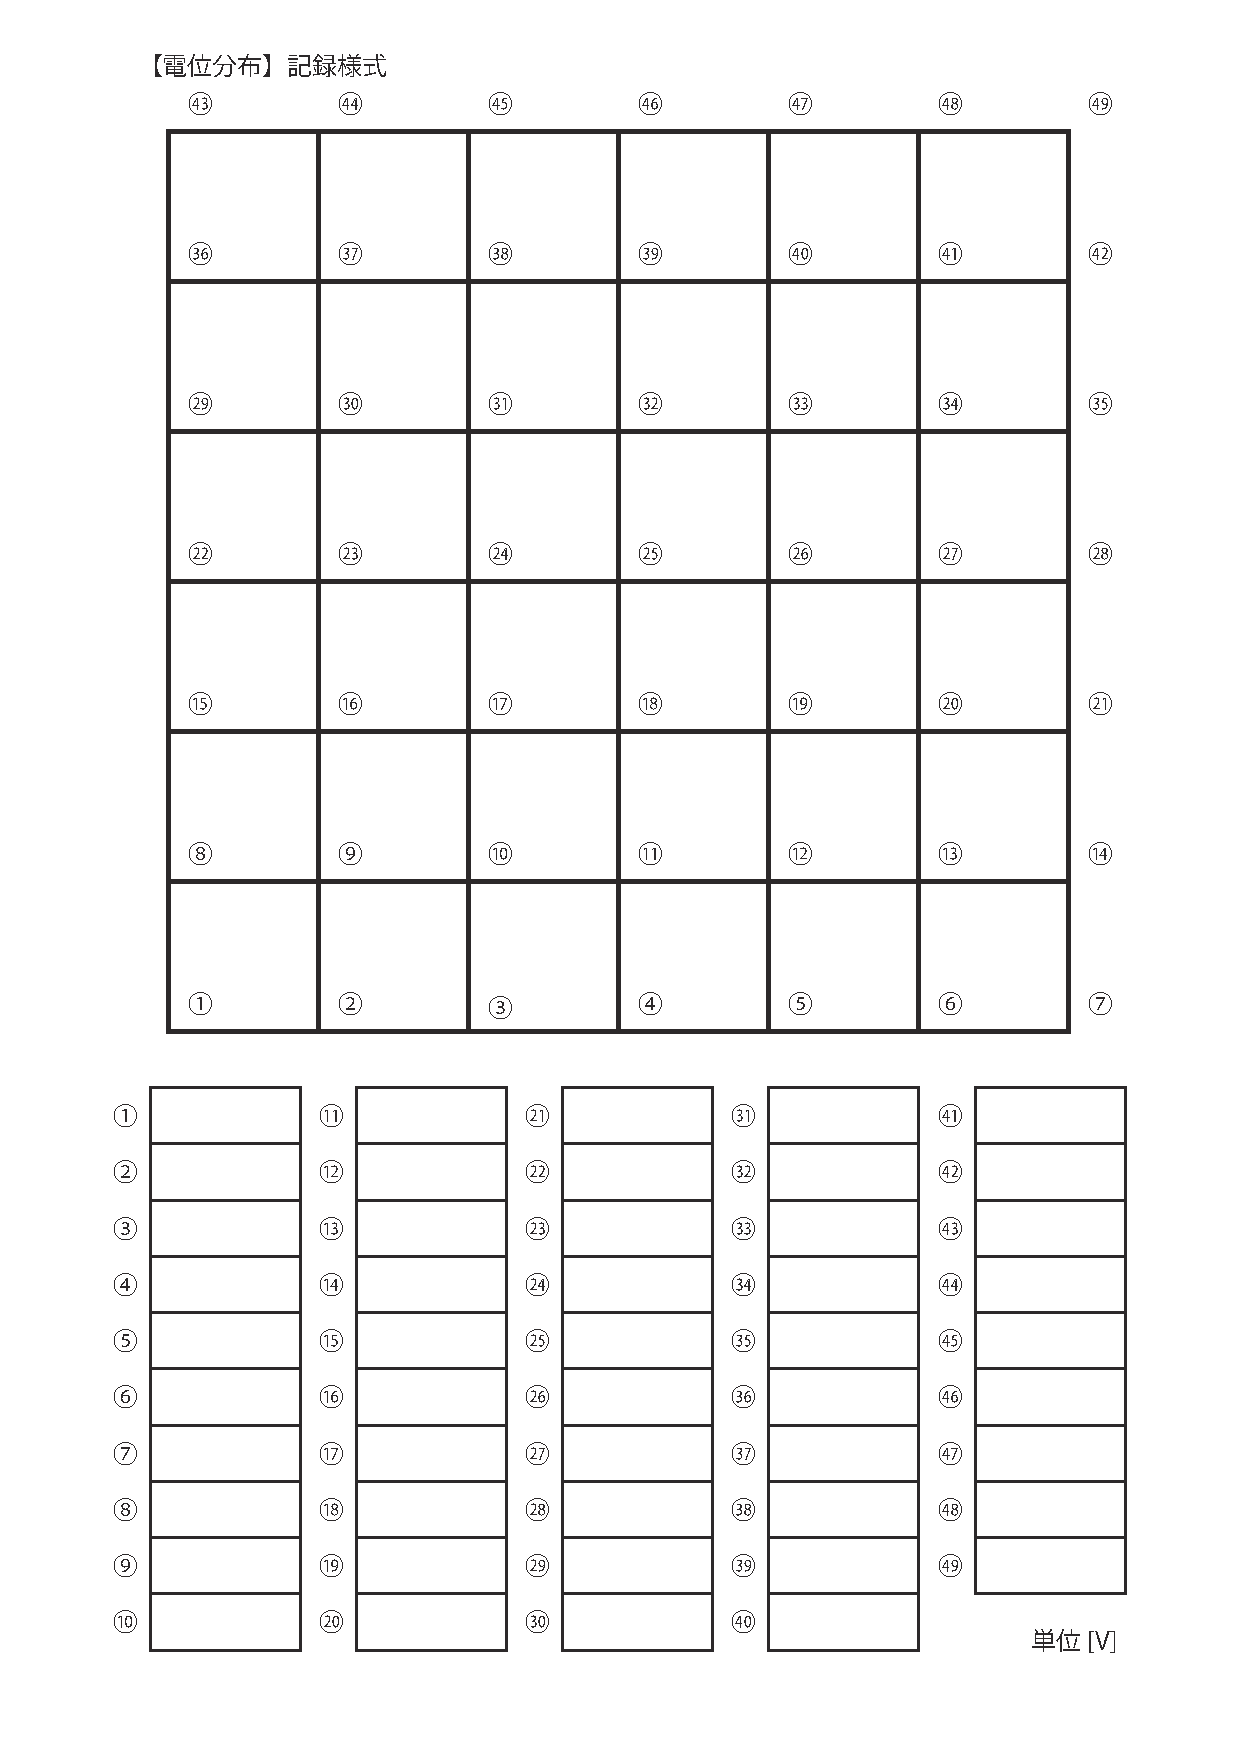
\includegraphics[scale=0.8]{./figure/E2.pdf}

\newpage

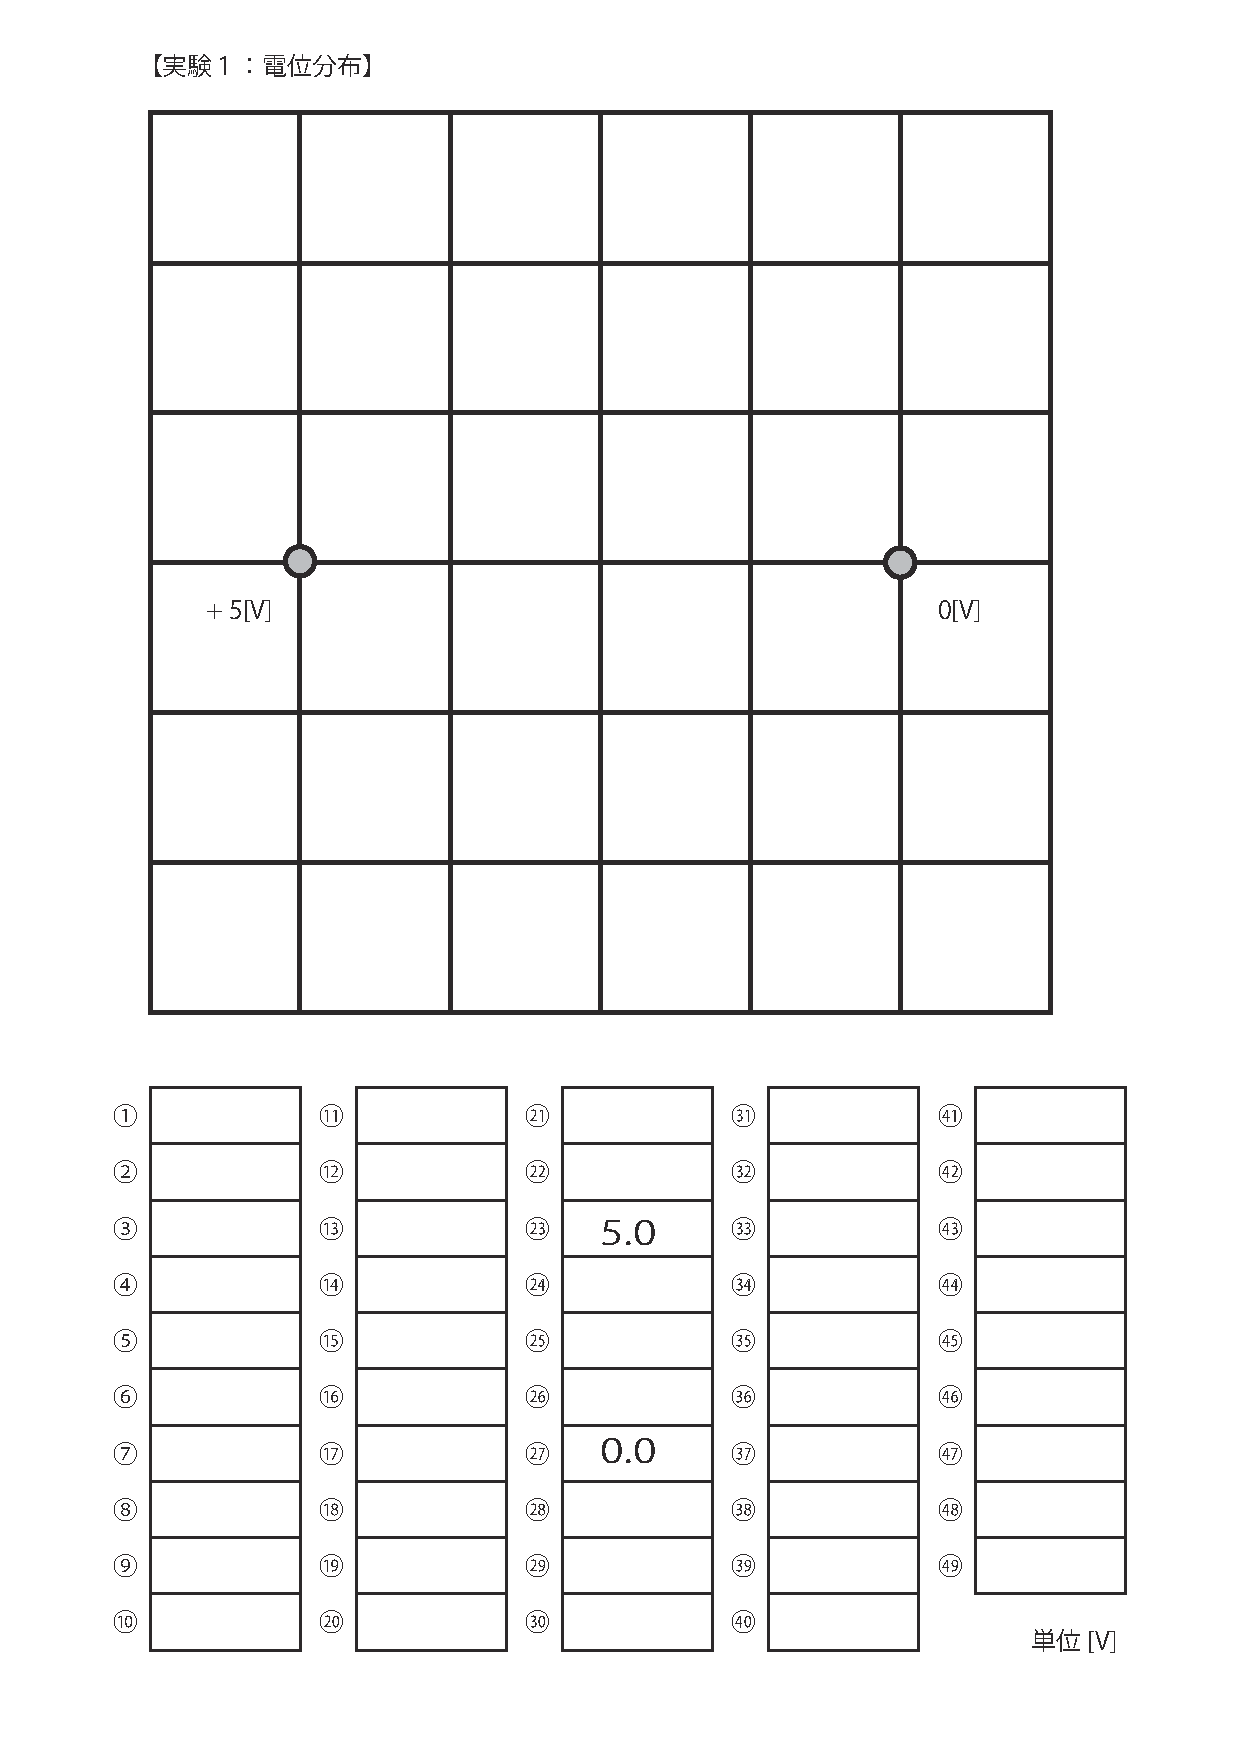
\includegraphics[scale=0.8]{./figure/E3.pdf}

\newpage

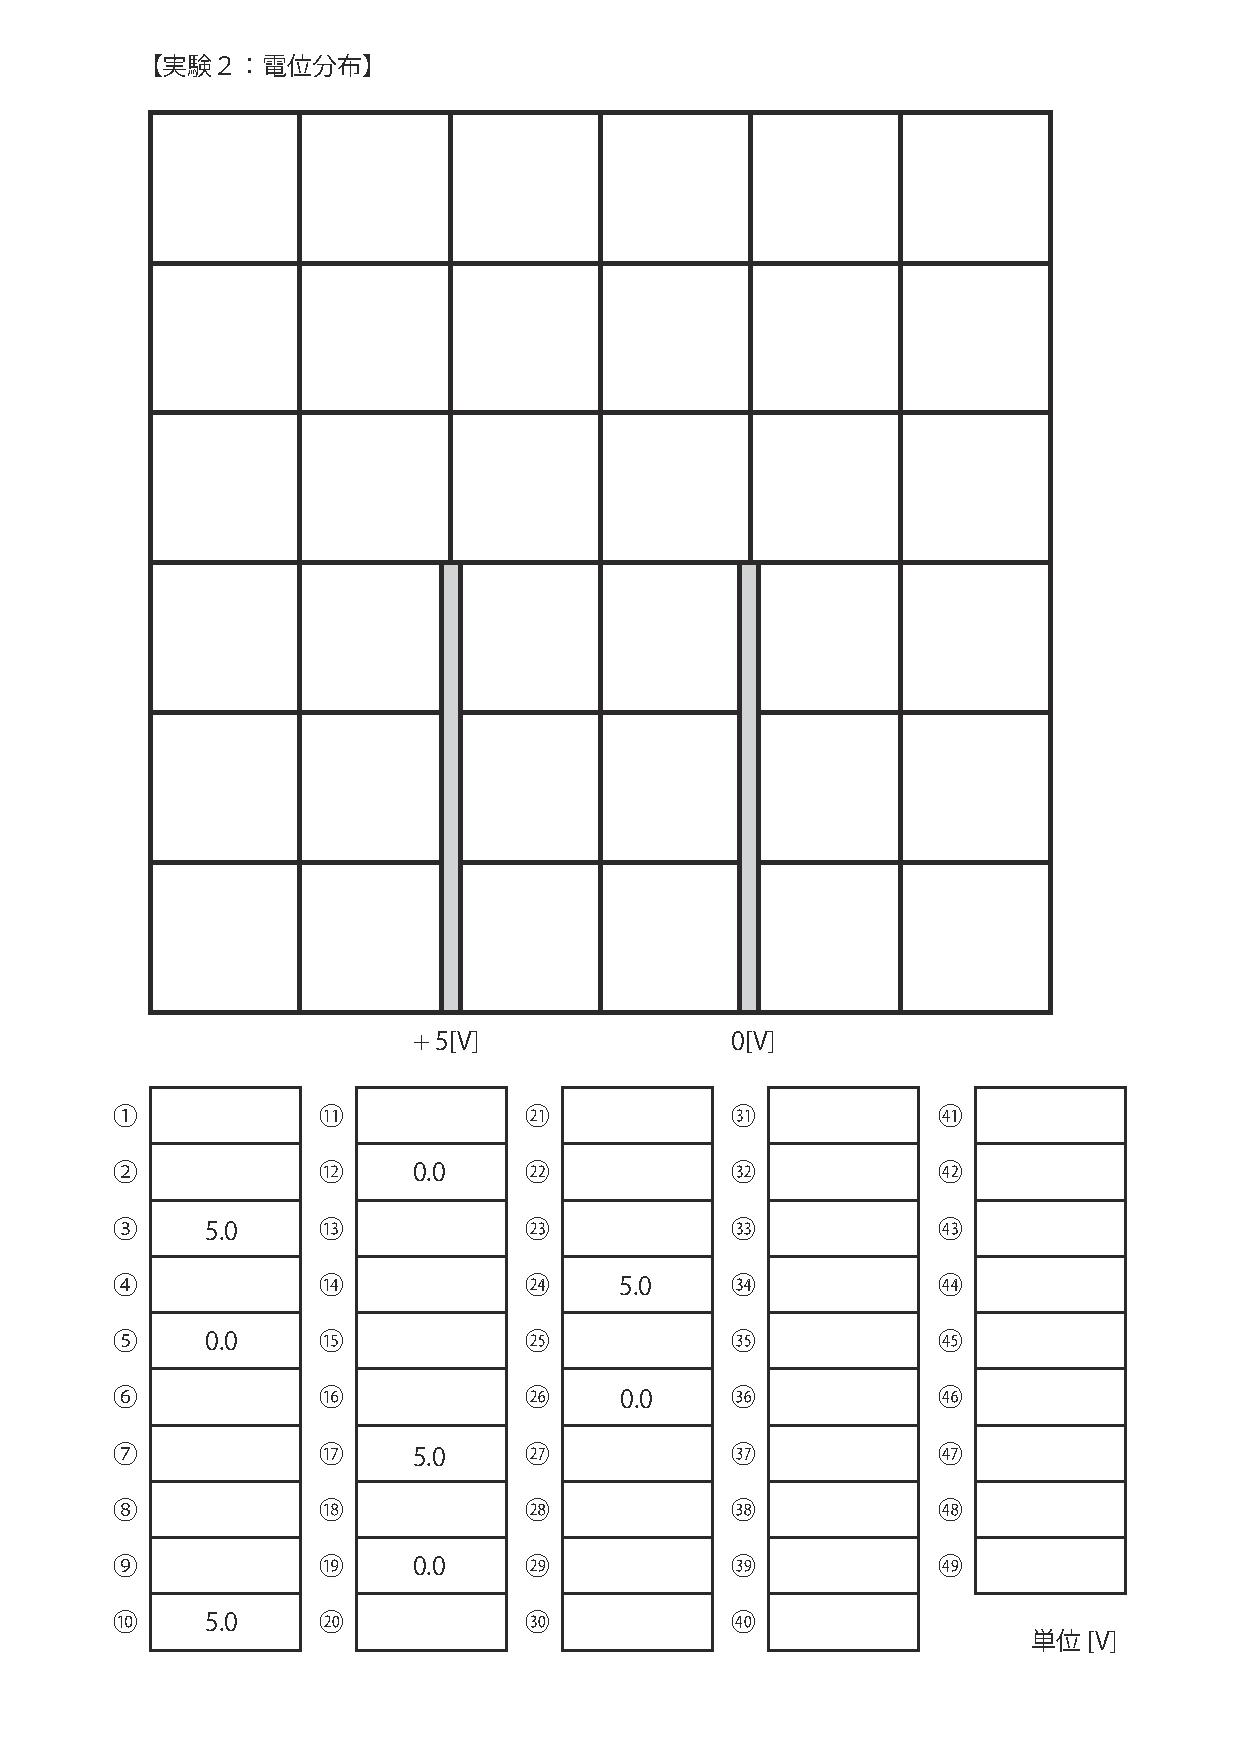
\includegraphics[scale=0.8]{./figure/E9.pdf}

\newpage

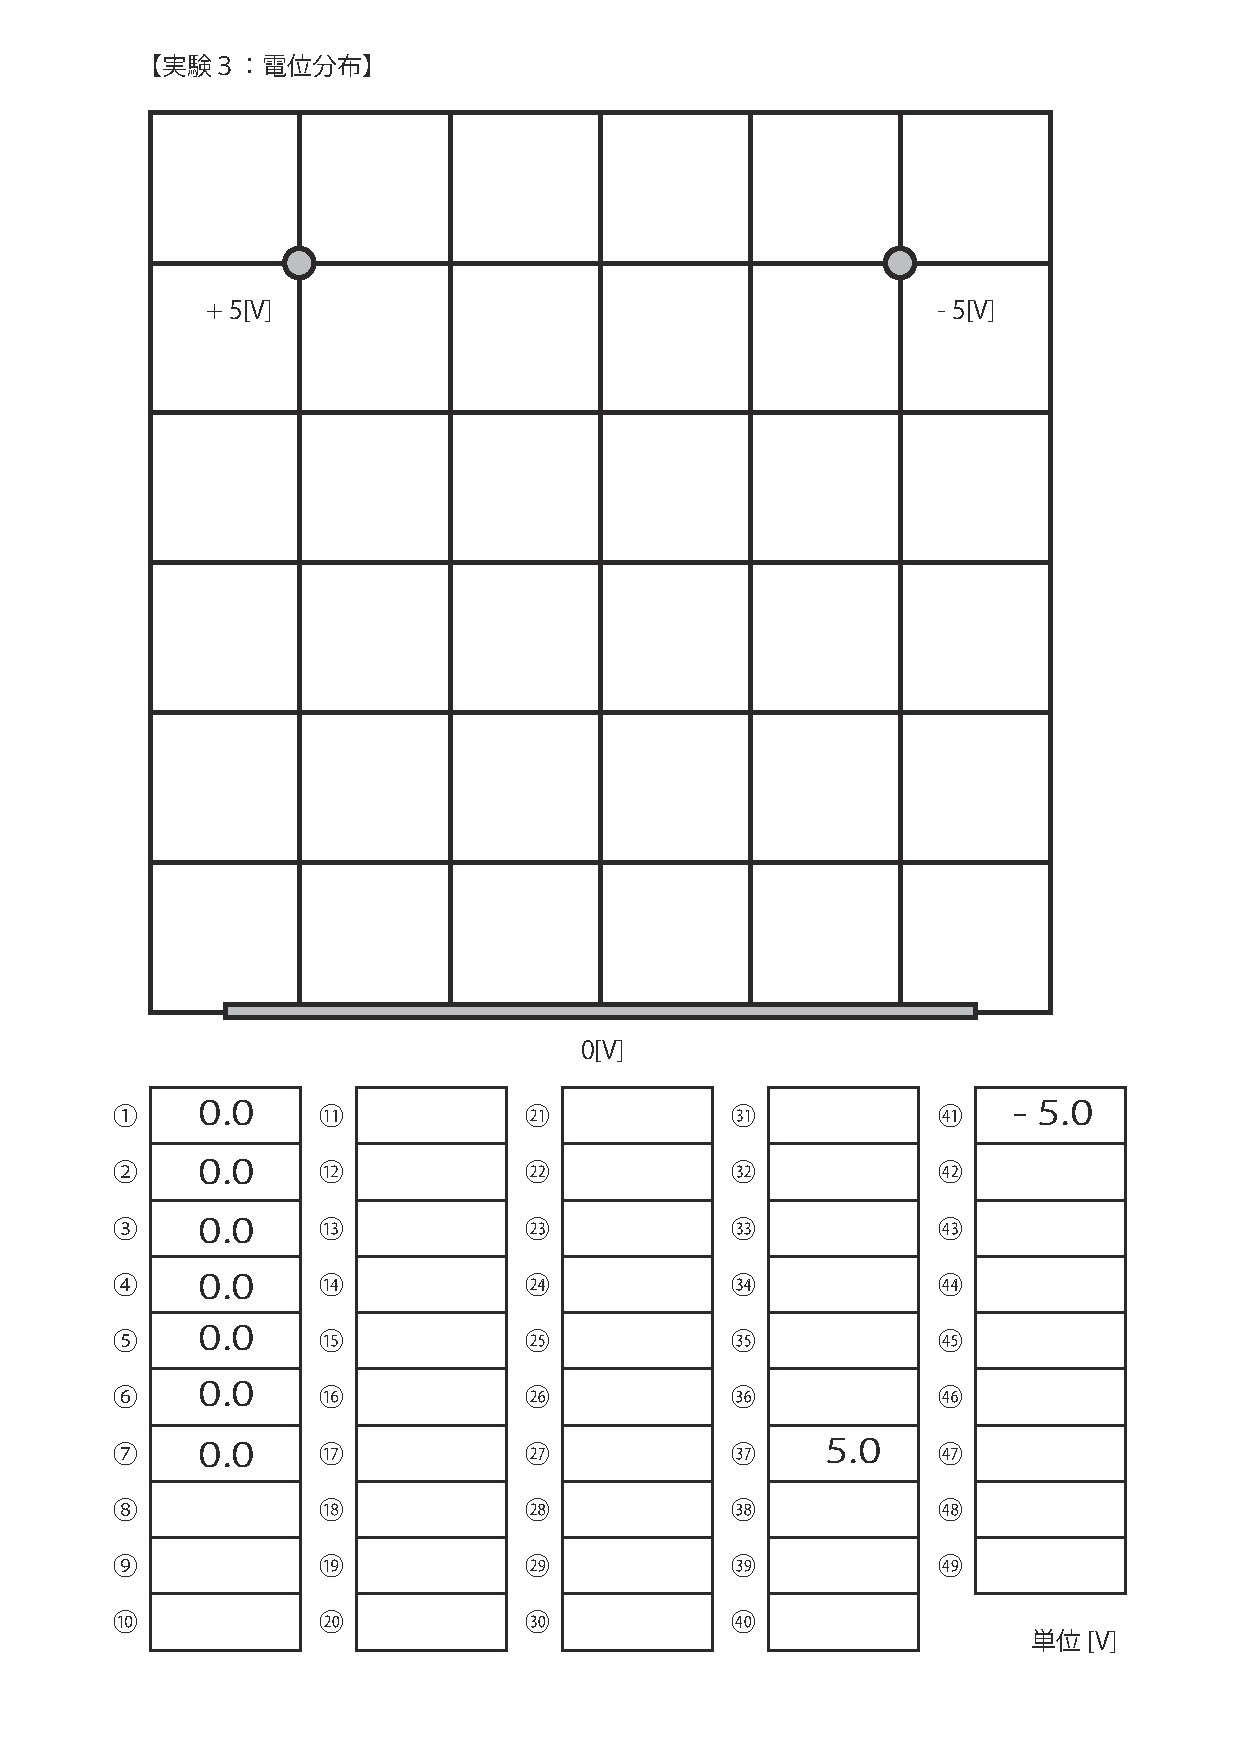
\includegraphics[scale=0.8]{./figure/E11.pdf}

\newpage

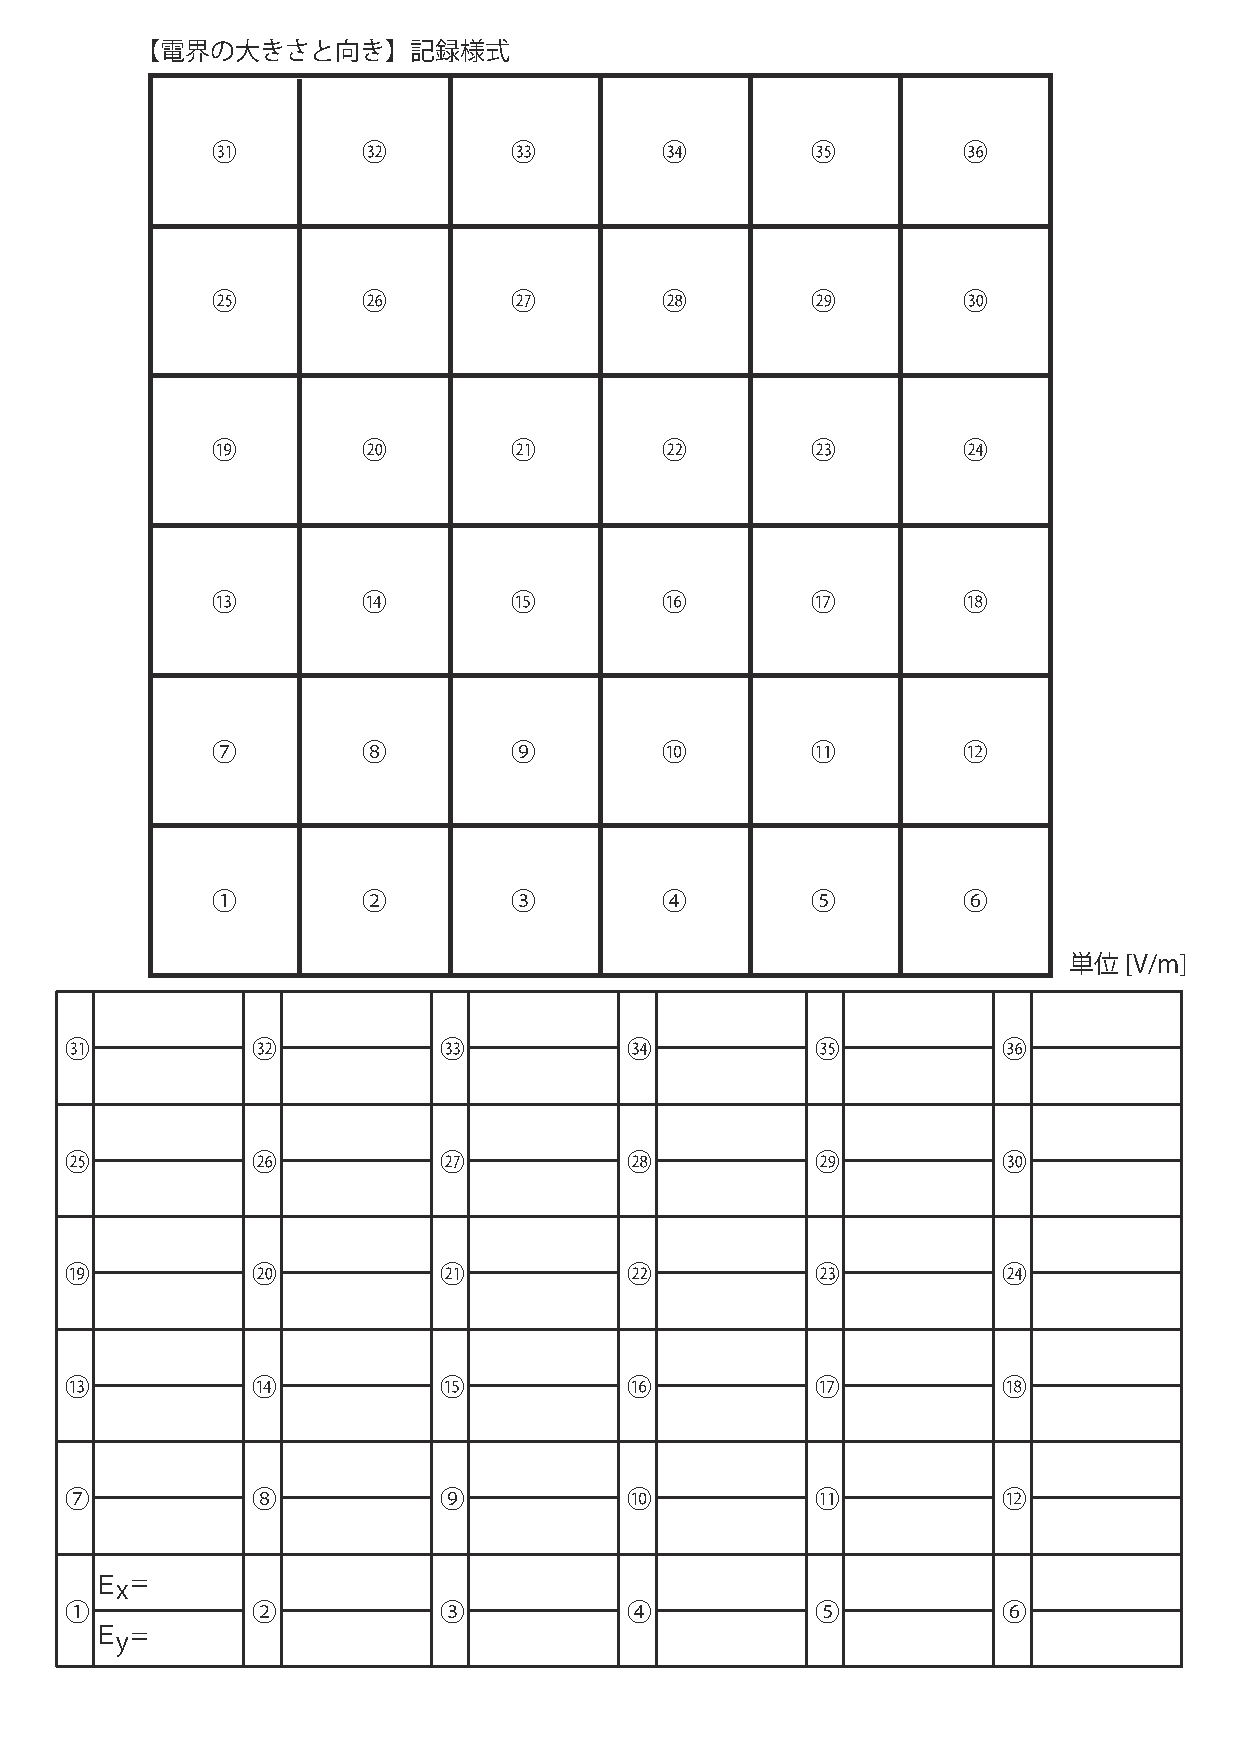
\includegraphics[scale=0.8]{./figure/E1.pdf}

\newpage

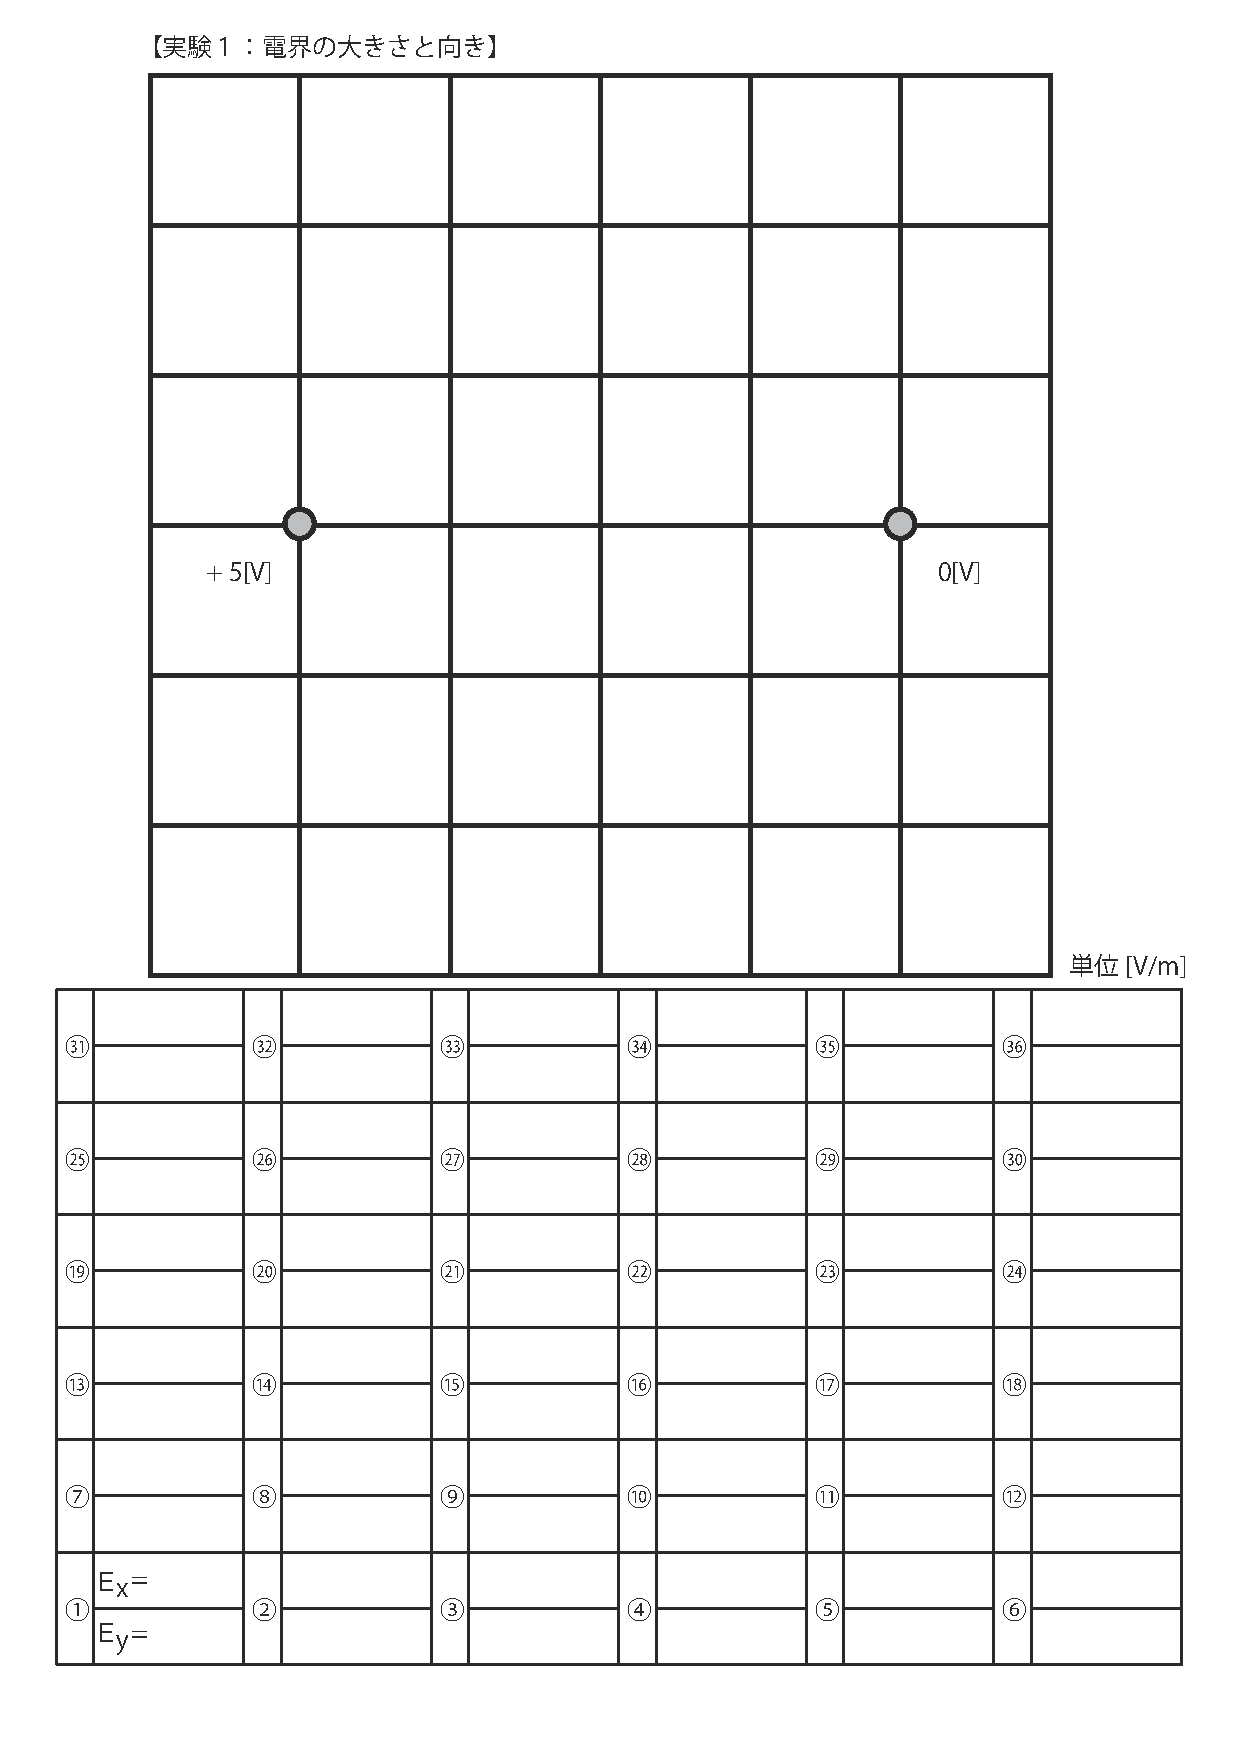
\includegraphics[scale=0.8]{./figure/E6.pdf}

\newpage

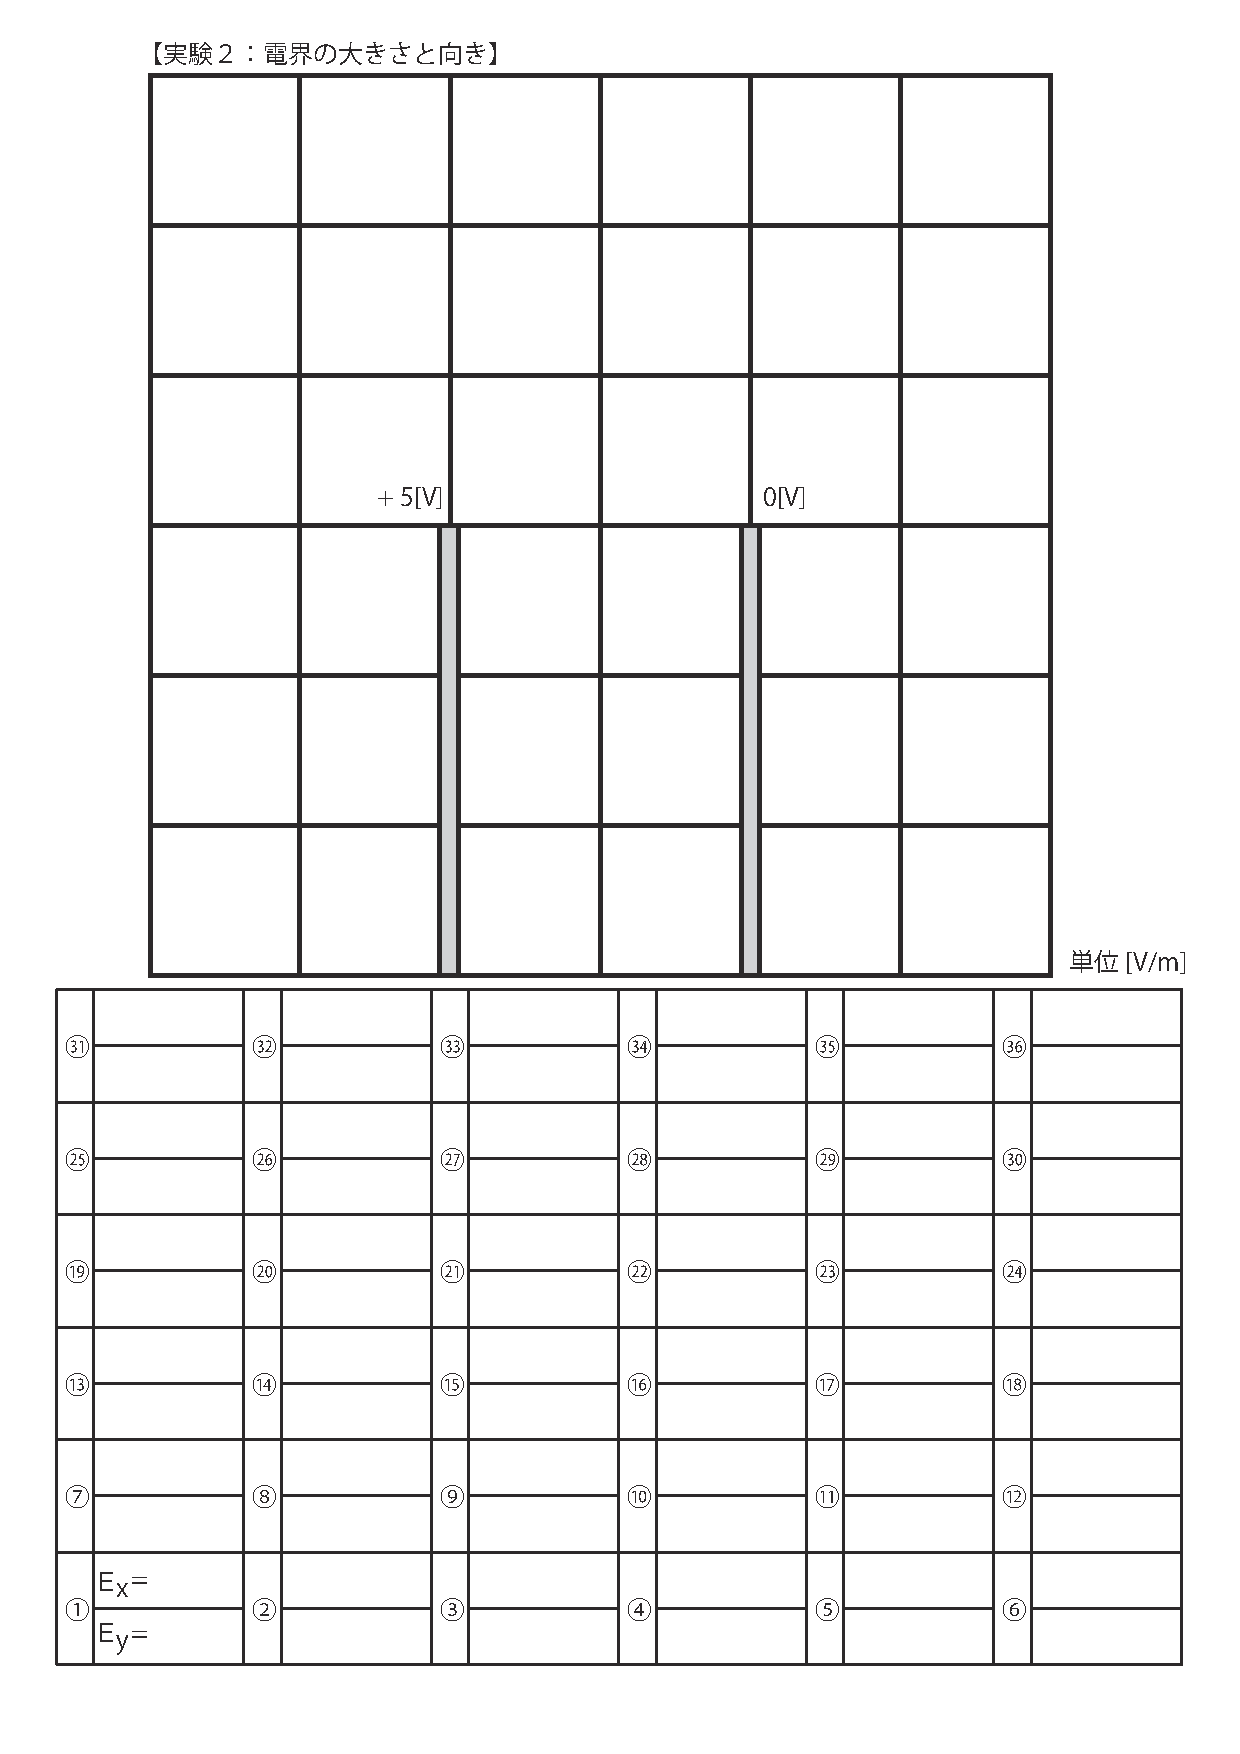
\includegraphics[scale=0.8]{./figure/E8.pdf}

\newpage

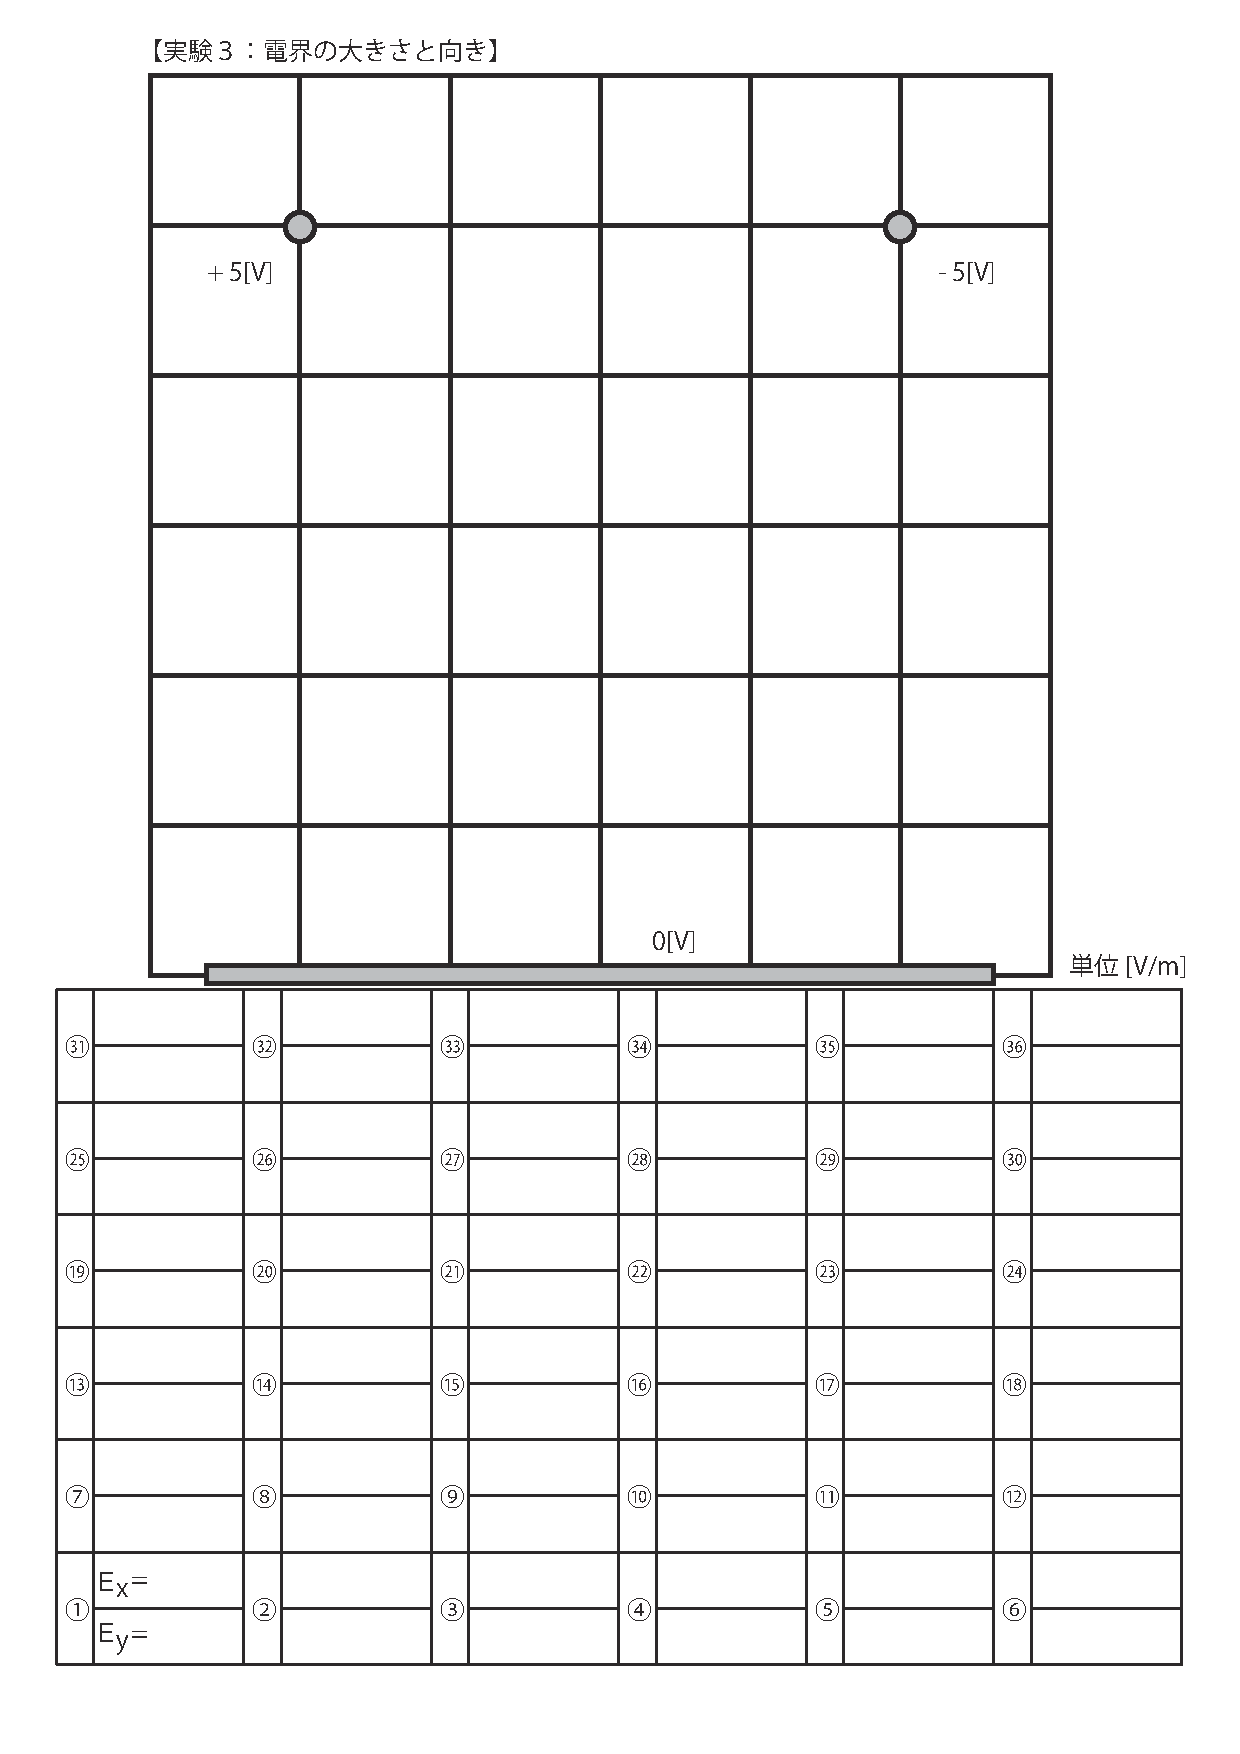
\includegraphics[scale=0.8]{./figure/E10.pdf}

\newpage

\lstinputlisting[caption=電位分布測定結果から等電位線の作図,label=prog1]{../src/prog1.py}

\newpage

\lstinputlisting[caption=電位分布測定結果から電気力線の作図,label=prog2]{../src/prog2.py}

\newpage

\lstinputlisting[caption=電位分布の模擬実験,label=prog3]{../src/prog3.py}

%
%\begin{thebibliography}{99}
%  \bibitem{1}
%\end{thebibliography}
%
% END DOCUMENT
\end{document}
%
